% Import default values & document settings
% Layout settings
\newcommand{\FIITdefaultFontSize}[0] {12pt}
\setcounter{secnumdepth}{3}
\setcounter{tocdepth}{3}

% Language settings
\newcommand{\FIITlanguage}[0] {slovak}
%\def\FIITlagEN{}

% Global texts
\newcommand{\FIITuniversity}[0] {Slovak University of Technology in Bratislava}
\newcommand{\FIITuniversitySK}[0] {Slovenská Technická Univerzita v Bratislave}
\newcommand{\FIITfaculty}[0] {Faculty of informatics and information technologies}
\newcommand{\FIITfacultySK}[0] {Fakulta informatiky a informačných technológií}
\newcommand{\FIITthesis}[0] {Master thesis}
\newcommand{\FIITthesisSK}[0] {Diplomová práca}
\newcommand{\FIITtitle}[0] {Centralized management and distribution of sensitive access data}
\newcommand{\FIITtitleSK}[0] {Centralizovaná správa a distribúcia citlivých prístupových údajov}
\newcommand{\FIITauthor}[0] {Bc. Adam Žúrek}
\newcommand{\FIITsupervisor}[0] {Ing. Ján Balážia PhD.}
\newcommand{\FIITevidenceNumber}[0] {FIIT-XXXX-XXXXX}
\newcommand{\FIITdate}[0] {June 2020}
\newcommand{\FIITdateSK}[0] {Jún 2020}
\newcommand{\FIITstudyProgram}[0] {Information security}
\newcommand{\FIITstudyProgramSK}[0] {Informačná bezpečnosť}
\newcommand{\FIITdegreeCourse}[0] {Informatics}
\newcommand{\FIITdegreeCourseSK}[0] {Informatika}
\newcommand{\FIITinstitute}[0] {Institute of Informatics and Software Engineering, FIIT STU, Bratislava}
\newcommand{\FIITinstituteSK}[0] {Ústav počítačového inžinierstva a aplikovanej informatiky, FIIT STU, Bratislava}
\newcommand{\FIITsignPlace}[0] {In Bratislava, }
\newcommand{\FIITsignPlaceSK}[0] {V Bratislave, }
\newcommand{\FIITsignDate}[0] {28.5.2020}


% Setup document
\documentclass[\FIITdefaultFontSize,a4paper,twoside,openright,\FIITlanguage]{book}

% Load all necessary packages
\usepackage[final]{pdfpages}
\usepackage[utf8]{inputenc}
\usepackage[T1]{fontenc}
\usepackage[a4paper]{geometry}
\usepackage[parfill]{parskip}
\usepackage{enumitem}
\usepackage{calc}
\usepackage{graphicx}
\usepackage{float}
\usepackage{longtable}
\usepackage{setspace}
\usepackage{tabularx}
\usepackage{fancyhdr}
\usepackage[backend=bibtex,sorting=none]{biblatex}
\usepackage{listing}
\usepackage{lscape}
\usepackage{afterpage}
\usepackage{hyperref}
\usepackage{bera}
\usepackage{listings}
\usepackage{xcolor}
\usepackage{lipsum}
\usepackage{lmodern}
\usepackage{fancyvrb}
\usepackage{tocloft}

% Remove unnecessary gap between paragraph if large figure is inserted after them
\raggedbottom

% Custom commands
\newcommand{\signaturespace}[2]{
  % #1 = width of the dotted line
  % #2 = legend
  \begingroup
  \renewcommand{\arraystretch}{0}
  \begin{tabular}[t]{cc}
  \hspace*{0pt}
  \cleaders\hbox{\kern.6pt.\kern.6pt}\hskip#1\relax
  \hspace*{0pt}
  \\[0.5cm]
  #2
  \end{tabular}
  \endgroup
}

\newcommand{\emptypage}{
\newpage
\thispagestyle{empty}
\mbox{}
\newpage
}

\renewcommand\appendixname{Príloha}
\renewcommand\chaptername{Kapitola}
\renewcommand{\figurename}{Obr.}

\definecolor{lightgray}{gray}{0.9}

\newcommand{\inlinecode}[1]{{\textbf{\colorbox{lightgray}{\textcolor{darkgray}{\footnotesize #1}}}}}

\colorlet{punct}{red!60!black}
\definecolor{background}{HTML}{EEEEEE}
\definecolor{delim}{RGB}{20,105,176}
\colorlet{numb}{magenta!60!black}

\lstdefinelanguage{json}{
    basicstyle=\normalfont\ttfamily,
    numbers=left,
    numberstyle=\scriptsize,
    stepnumber=1,
    numbersep=8pt,
    showstringspaces=false,
    breaklines=true,
    frame=lines,
    backgroundcolor=\color{background},
    literate=
     *{0}{{{\color{numb}0}}}{1}
      {1}{{{\color{numb}1}}}{1}
      {2}{{{\color{numb}2}}}{1}
      {3}{{{\color{numb}3}}}{1}
      {4}{{{\color{numb}4}}}{1}
      {5}{{{\color{numb}5}}}{1}
      {6}{{{\color{numb}6}}}{1}
      {7}{{{\color{numb}7}}}{1}
      {8}{{{\color{numb}8}}}{1}
      {9}{{{\color{numb}9}}}{1}
      {:}{{{\color{punct}{:}}}}{1}
      {,}{{{\color{punct}{,}}}}{1}
      {\{}{{{\color{delim}{\{}}}}{1}
      {\}}{{{\color{delim}{\}}}}}{1}
      {[}{{{\color{delim}{[}}}}{1}
      {]}{{{\color{delim}{]}}}}{1},
}

\bibliography{bibliography}

% Page design
\pagestyle{fancy}
\lhead{\nouppercase{\leftmark}}
\chead{}
\rhead{}
\lfoot{}
\cfoot{\thepage}
\rfoot{}

\begin{document}

% Initialize document
% Layout
\setstretch{1.5}

% Bibliography
\ifx\FIITlagEN\undefined
\defbibheading{references}[Zoznam použitej literatúry]{
  \chapter*{#1}
  \markboth{#1}{#1}
}
\defbibheading{referencessec}[Zoznam použitej literatúry]{
  \section*{#1}
  \markboth{#1}{#1}
}
\else
\defbibheading{references}[References]{
  \chapter*{#1}
  \markboth{#1}{#1}
}
\defbibheading{referencessec}[References]{
  \section*{#1}
  \markboth{#1}{#1}
}
\fi

% Syntax highlighting
\colorlet{punct}{red!60!black}
\definecolor{background}{HTML}{EEEEEE}
\definecolor{delim}{RGB}{20,105,176}
\colorlet{numb}{magenta!60!black}

\lstdefinelanguage{json}{
    basicstyle=\normalfont\ttfamily,
    numbers=left,
    numberstyle=\scriptsize,
    stepnumber=1,
    numbersep=8pt,
    showstringspaces=false,
    breaklines=true,
    frame=lines,
    backgroundcolor=\color{background},
    literate=
     *{0}{{{\color{numb}0}}}{1}
      {1}{{{\color{numb}1}}}{1}
      {2}{{{\color{numb}2}}}{1}
      {3}{{{\color{numb}3}}}{1}
      {4}{{{\color{numb}4}}}{1}
      {5}{{{\color{numb}5}}}{1}
      {6}{{{\color{numb}6}}}{1}
      {7}{{{\color{numb}7}}}{1}
      {8}{{{\color{numb}8}}}{1}
      {9}{{{\color{numb}9}}}{1}
      {:}{{{\color{punct}{:}}}}{1}
      {,}{{{\color{punct}{,}}}}{1}
      {\{}{{{\color{delim}{\{}}}}{1}
      {\}}{{{\color{delim}{\}}}}}{1}
      {[}{{{\color{delim}{[}}}}{1}
      {]}{{{\color{delim}{]}}}}{1},
}


% Cover & title page
%%%%%%%%%%%%%%%%%%%%%%%%%%%%%%%%%%%%%%%%%%%%%%%%%%%%%%%%%%%%%%%%%%%%%%%%%%%%%%%%%%%%%%%%
%%
%% Cover page
%%
%%%%%%%%%%%%%%%%%%%%%%%%%%%%%%%%%%%%%%%%%%%%%%%%%%%%%%%%%%%%%%%%%%%%%%%%%%%%%%%%%%%%%%%%
\begin{center}
\thispagestyle{empty}
\ifx\FIITlagEN\undefined
{\Large \FIITuniversitySK}
\else
{\Large \FIITuniversity}
\fi
\par\end{center}{\Large \par}

\begin{center}
\ifx\FIITlagEN\undefined
{\Large \FIITfacultySK}
\else
{\Large \FIITfaculty}
\fi
\par\end{center}{\Large \par}

\smallskip{}

\begin{center}
\FIITevidenceNumber
\par\end{center}
\vfill{}

\begin{center}
{\Large \FIITauthor}
\par\end{center}{\Large \par}

\medskip{}


\begin{center}
\ifx\FIITlagEN\undefined
{\LARGE \FIITtitleSK}
\else
{\LARGE \FIITtitle}
\fi
\par\end{center}{\huge \par}

\medskip{}


\begin{center}

\ifx\FIITlagEN\undefined
{\Large \FIITthesisSK}
\else
{\Large \FIITthesis}
\fi
\par\end{center}{\Large \par}

\vfill{}


\ifx\FIITlagEN\undefined
Vedúci práce: \FIITsupervisor
\else
Supervisor: \FIITsupervisor
\fi

\medskip{}

\ifx\FIITlagEN\undefined
\FIITdateSK
\else
\FIITdate
\fi

\pagenumbering{roman}
\emptypage

%%%%%%%%%%%%%%%%%%%%%%%%%%%%%%%%%%%%%%%%%%%%%%%%%%%%%%%%%%%%%%%%%%%%%%%%%%%%%%%%%%%%%%%%
%%
%% Thesis title page
%%
%%%%%%%%%%%%%%%%%%%%%%%%%%%%%%%%%%%%%%%%%%%%%%%%%%%%%%%%%%%%%%%%%%%%%%%%%%%%%%%%%%%%%%%%
\begin{center}
\thispagestyle{empty}
\ifx\FIITlagEN\undefined
{\Large \FIITuniversitySK}
\else
{\Large \FIITuniversity}
\fi
\par\end{center}{\Large \par}

\begin{center}
\ifx\FIITlagEN\undefined
{\Large \FIITfacultySK}
\else
{\Large \FIITfaculty}
\fi
\par\end{center}{\Large \par}

\smallskip{}

\begin{center}
\FIITevidenceNumber
\par\end{center}
\vfill{}

\begin{center}
{\Large \FIITauthor}
\par\end{center}{\Large \par}

\medskip{}


\begin{center}
\ifx\FIITlagEN\undefined
{\LARGE \FIITtitleSK}
\else
{\LARGE \FIITtitle}
\fi
\par\end{center}{\huge \par}

\medskip{}


\begin{center}

\ifx\FIITlagEN\undefined
{\Large \FIITthesisSK}
\else
{\Large \FIITthesis}
\fi
\par\end{center}{\Large \par}

\vfill{}


\ifx\FIITlagEN\undefined
Študijný program: \quad\quad\quad\FIITstudyProgramSK

Študijný odbor: \quad\quad\quad\quad\FIITdegreeCourseSK

Miesto vypracovania:\quad\quad\FIITinstituteSK

Vedúci práce: \quad\quad\quad\quad\quad\FIITsupervisor
\else
Study program:              \quad\FIITstudyProgram

Degree course:              \quad\FIITdegreeCourse

Place of elaboration:       \quad\FIITinstitute

Supervisor:                 \quad\FIITsupervisor
\fi

\medskip{}

\ifx\FIITlagEN\undefined
\FIITdateSK
\else
\FIITdate
\fi

\emptypage


% Thesis assignment
\newpage
\thispagestyle{empty}

\includepdf[pages=1,scale=1]{assets/zadanie}
\newpage
\emptypage

% Thesis proposal assignment
\newpage
\thispagestyle{empty}

\includepdf[pages=1,scale=1]{assets/navrh_zadanie}

\includepdf[pages=2,scale=1]{assets/navrh_zadanie}
\newpage

% Declaration of honor
\thispagestyle{empty}

\vspace*{\fill}

\section*{Čestné prehlásenie}

Čestne vyhlasujem, že som túto prácu vypracoval samostatne, na základe
konzultácií a s použitím uvedenej literatúry.

\FIITsignPlaceSK \FIITsignDate
\hspace*{\fill} \signaturespace{5cm}{\FIITauthor}

\emptypage


% Acknowledgements
\thispagestyle{empty}

\vspace*{\fill}

\ifx\FIITlagEN\undefined
\section*{Poďakovanie}
\else
\section*{Special thanks}
\fi

\lipsum[4]

\emptypage


% Annotation
%%%%%%%%%%%%%%%%%%%%%%%%%%%%%%%%%%%%%%%%%%%%%%%%%%%%%%%%%%%%%%%%%%%%%%%%%%%%%%%%%%%%%%%%
%%
%% Slovak annotation
%%
%%%%%%%%%%%%%%%%%%%%%%%%%%%%%%%%%%%%%%%%%%%%%%%%%%%%%%%%%%%%%%%%%%%%%%%%%%%%%%%%%%%%%%%%
\newpage
\thispagestyle{plain}
\begin{flushleft}
\begin{Large}
\textbf{Anotácia} \\
\end{Large}
Slovenská technická univerzita v Bratislave \\
FAKULTA INFORMATIKY A INFORMAČNÝCH TECHNOLÓGIÍ\vspace{0.6cm}
\noindent
	\textrm{
	    \begin{normalsize}
	    \begin{tabular}{@{}ll@{}}
			Študijný program: & \FIITstudyProgramSK\\
			Diplomová práca: & \FIITtitleSK \\
			Autor: & \FIITauthor \\
			Vedúci práce: & \FIITsupervisor \\
			Jún,\ 2020
	    \end{tabular}
	  	\end{normalsize}
	}
\noindent
\end{flushleft}

Každá softvérová firma musí riešiť otázky, ktoré vyplívajú z problémov ohľadom informačnej bezpečnosti. Takéto typy problémov
by nemali byť prehliadané, z dôvodu možných následkov v podobe výskytu bezpečnostných rizík. Obsah práce sa v prvom rade
zameriava na analýzu ich možných výskytov vo firemnom prostredí, s možnosťami ich následného odstránenia, prípadne minimalizovania
podľa overených bezpečnostných riešení používaných v súčasnosti. Tieto riešenia sú následne rozobrané z pohľadu manažmentu
informačnej bezpečnosti a prislúchajúcim štandardom. Výstupom práce je softvérový produkt, ktorý bude využívať súčasné a
overené metódy na odstránenie alebo minimalizovanie daných rizík v praxi. Produkt sa bude zameriavať na autorizáciu, ktorá
bude vyplívať z presne stanovenej hierarchie softvérovej firmy. Dôležitou súčasťou je taktiež správna a bezpečná autentifikácia
spolu so správnym ukladaním a manažovaním citlivých údajov. Tieto údaje budú slúžiť ako prístupové kľúče ku koncovým zariadeniam
zákazníkov, pričom cieľom je na tieto zariadenia bezpečne a automatizovane nasadiť finálny produkt. Z tohto pohľadu je dôležité
brať do úvahy aj možné hrozby, ktorými môžu byť kompromitovaní aj samotní zákazníci. Z toho dôvodu je umožnený iba dočasný
prístup ku koncovým zariadeniam, kde samotné prístupové údaje budú dynamicky menené na oboch stranách komunikujúcich uzľov.
\emptypage

%%%%%%%%%%%%%%%%%%%%%%%%%%%%%%%%%%%%%%%%%%%%%%%%%%%%%%%%%%%%%%%%%%%%%%%%%%%%%%%%%%%%%%%%
%%
%% English annotation
%%
%%%%%%%%%%%%%%%%%%%%%%%%%%%%%%%%%%%%%%%%%%%%%%%%%%%%%%%%%%%%%%%%%%%%%%%%%%%%%%%%%%%%%%%%
\newpage
\thispagestyle{plain}
\begin{flushleft}
\begin{Large}
\textbf{Annotation} \\
\end{Large}
Slovak University of Technology Bratislava \\
FACULTY OF INFORMATICS AND INFORMATION TECHNOLOGIES\vspace{0.6cm}
\noindent
	\textrm{
	    \begin{normalsize}
	    \begin{tabular}{@{}ll@{}}
			Study program: & \FIITstudyProgram\\
			Master thesis: & \FIITtitle \\
			Author: & \FIITauthor \\
			Supervisor: & \FIITsupervisor \\
			June,\ 2020
	    \end{tabular}
	  	\end{normalsize}
	}
\noindent
\end{flushleft}
Every software company has to deal with issues that arise from information security issues. These types of problems should
not be overlooked, due to the possible consequences in terms of security risks. The content of the work is primarily focused
on the analysis of their possible occurrences in the corporate environment, with the possibility of their subsequent removal,
or minimization according to proven security solutions currently used. These solutions are then analyzed from the perspective
of information security management and the relevant standards. The output of the work is a software product that will use
current and proven methods to eliminate or minimize the risks in practice. The product will focus on authorization, which
will result from a well-defined hierarchy of the software company. Correct and secure authentication is also an important
part, along with the correct storage and management of sensitive data. This data will serve as access keys to customers'
end devices, with the goal of securely and automatically deploying the final product to those devices. From this point
of view, it is important to take into account the possible threats that may compromise customers themselves. For this
reason, only temporary access to the terminal devices is allowed, where the access data itself will be dynamically
changed on both sides of the communicating nodes.
\emptypage


% Table of contents
\renewcommand{\contentsname}{Obsah}
\tableofcontents
\pagebreak

% List of figures
\renewcommand{\listfigurename}{Zoznam obrázkov}
\listoffigures
\pagebreak

% List of abbreviations
\lhead{Zoznam použitých skratiek}

\chapter*{Zoznam použitých skratiek}\label{ch:zoznam-pouzitych-skratiek}

\textbf{CIA}   - Confidentiality, Integrity, Availability \\
\textbf{GDPR}  - General Data Protection Regulation \\
\textbf{ISMS}  - Information Security Management System \\
\textbf{MITM}  - Man in the Middle\\
\textbf{PDCA}  - Plan - Do - Check - Act\\
\textbf{RBAC}  - Role Based Access Control\\
\textbf{ABAC}  - Attribute Based access control\\
\textbf{XACML} - eXtensible Access Control Markup Language\\
\textbf{LDAP}  - Lightweight Directory Access Protocol\\
\textbf{HTTPS} - Hypertext Transfer Protocol Secure\\
\textbf{TLS}   - Transport Layer Security\\
\textbf{JWT}   - JSON Web Token\\
\textbf{OAUTH} - Open standard for access delegation\\
\textbf{SSH}   - Secure Shell\\
\textbf{SFTP}  - SSH File Transfer Protocol\\
\textbf{TCP}   - Transmission Control Protocol\\
\textbf{IP}    - Internet Protocol\\
\textbf{AES}   - Advanced Encryption Standard\\
\textbf{NSA}   - National Security Agency\\
\textbf{NIST}  - National Institute of Standards and Technology\\
\textbf{SIV}   - Synthetic Initialization Vector\\
\textbf{CFB}   - Cipher Feedback\\
\textbf{AWS}   - Amazon Web Services\\
\textbf{CMK}   - Customer Master Key\\
\textbf{EER}   - Enhanced Entity-Relationship\\
\textbf{PKI}   - Public Key Infrastructure\\
\textbf{CA}    - Certification Authority\\
\textbf{OTP}   - One Time Password\\
\textbf{ORM}   - Object-relational Mapping\\


% Enable page numbering
\pagenumbering{arabic}
\lhead{\nouppercase{\leftmark}}

% Begin refferences segment
\renewcommand\bibname{Reference}
\begin{refsegment}

\chapter{Úvod}\label{ch:úvod}

V súčasnej dobe je pre väčšinu informatikov dostupná veľká škála možností, akým spôsobom sa vedia v praxi angažovať.
Jedným z populárnych spôsobov je možnosť založenia vlastnej softvérovej firmy.
S narastajúcou potrebou využívania softvérových služieb a digitalizácie sa taktiež zvýšil počet firiem poskytujúcich tieto riešenia.
Príkladom je Nemecko, kde od roku 2008 po rok 2017 narástol počet softvérových firiem o približne o 24\%~\cite{CompaniesGerman}.
V škótsku bol nárast počtu v rovnakom časovom období až o 60\%~\cite{SoftwareBusiness}, pričom majoritnými typmi nových
firiem sú stredné a malé podniky~\cite{CompaniesScotch}.
Na to, aby softvérová firma zabezpečila so zákazníkom profesionálny a adekvátny prístup, je nutné dodržovať viacero noriem.
Jedným zo základných princípov softvérového inžinierstva sú vlastnosti softvéru, ako napríklad spoľahlivosť alebo integrita.
Na druhej strane korektný postup pri tvorbe softvéru nie je jediný z dôležitých čŕt dobrej a úspešnej firmy.
Medzi ďalšie dôležité aspekty patrí aj vnútro firemné zriadenie.
Z tohto hľadiska je veľmi dôležité dbať ohľad na bezpečnosť firmy a hlavne aj jej zákazníkov.
Práve z hľadiska informačnej bezpečnosti~\cite{IB}, vzniká v softvérových firmách veľa otázok súvisiacich s bezpečnostnými problémami.
Prehliadanie, alebo ignorovanie takýchto výstražných znamení, najmä v spomínaných firmách s menším vzrastom má vo väčšine
prípadov za následok vznik bezpečnostných rizík.
Takéto riziká je možné z pohľadu potenciálneho útočníka zneužiť, čím vie softvérovej firme, v určitých prípadoch aj jej
zákazníkom napáchať nemalé škody.
Takéto typy škôd môžu mať za následok stratu finančných prostriedkov, zvýšiť čas potrebný na dodanie finálneho
produktu, poškodiť povesť firmy, prípadne kompromitovať koncové zariadenia zákazníkov.
Čo má teda za následok prehliadanie jednotlivých bezpečnostných problémov u väčšiny softvérových firiem?
Aké sú v súčasnej dobe možnosti dané problémy v praxi riešiť v súlade s manažmentom informačnej bezpečnosti?
V akých prípadoch sa dané problémy vyskytujú a aké konkrétne riziká z nich vyplývajú?
V prvom rade našou úlohou bude odhaliť veľkú časť hrozieb zaoberajúcich sa predovšetkým oblasťou „kontaktu“ medzi softvérovou firmou a zákazníkom.
Daná oblasť je podmienená presne navrhnutými a špecifikovanými bezpečnostnými
postupmi, ktoré sú nevyhnutné pre správnu a bezpečnú manipuláciu s citlivými údajmi zákazníkov.
Medzi postupy napríklad patrí presne stanovená hierarchia medzi zamestnancami v internom prostredí firmy v súlade s manažmentom informačnej bezpečnosti.
Z toho vyplýva, že na správnu a bezpečnú manipuláciu s citlivými prostriedkami zákazníkov budú musieť byť presne stanovené
bezpečnostné pravidlá firmy.
Náplňou našej práce je teda navrhnúť bezpečnostný informačný systém, ktorý bude dodržiavanie navrhnutých firemných
pravidiel striktne validovať s cieľom bezpečného uloženia firemných citlivých údajov, kde napríklad patria prístupové
údaje ku koncovým zariadeniam zákazníkov.
Medzi dôležité bezpečnostné oblasti riešenia bude patriť správna a bezpečná autentifikácia, autorizácia, ukladanie
citlivých údajov a informácií v súlade s ochranou osobných údajov (GDPR)~\cite{GDPR}.
Medzi ďalšie témy, ktorými sa bude naša práca zaoberať sú bezpečné komunikačné protokoly na výmenu prístupových údajov a ich validáciu.
Automatizácia nasadenia finálnych softvérových produktov na koncové zariadenia je taktiež jedným z cieľov našej práce.
Vysokou prioritou riešenia je jeho vysoká modularita~\cite{Modularity} a možná jednoduchá rozšíriteľnosť~\cite{Scalability}.

\chapter{Analýza}\label{ch:analýza}

\section{Bezpečnostné hrozby}\label{sec:podsekcia-1}
\par Z hľadiska bezpečnosti musí väčšina firiem čeliť viacerým hrozbám. V ideálnom prostredí a vo veľkých softvérových
firmách slúži na analýzu bezpečnostných hrozieb takzvaný Systém riadenia informačnej bezpečnosti
(Information Security Management System - ISMS) podľa normy ISO 27000~\cite{ISO27001:2013}. Úlohou takéhoto systému je
definovanie a spravovanie rizík, ktoré môžu vyplívať z hrozieb a zraniteľností. Dôležitou časťou je ochrana aktív s vysokou
hodnotou. Na obrázku~\ref{obr_1} je možné vidieť schému riadenia takýchto rizík.

\par Medzi najzákladnejšie bezpečnostné problémy napríklad patrí nezabezpečený prístup k jednotlivým projektom medzi zamestnancami.
K jednotlivým projektom v softvérovej firme by mali mať prístup iba tí zamestnanci, ktorí sa podieľajú na jeho správe a implementácii.
Vystavenie prístupových údajov, rôznych informácií o zákazníkovi a jeho používateľoch neprislúchajúcemu zamestnancovi,
môže spôsobiť veľa bezpečnostných rizík. Napríklad zamestnanec môže zneužiť dátové úložisko nachádzajúce sa v produkcii.
Zamestnanec môže týmto spôsobom  napríklad získať citlivé informácie o tržbách zákazníka alebo adrese. Taktiež vie získať
prístupové dáta k jeho koncovým zariadeniam a kompromitovať ich. Týmto bezpečnostným rizikám prislúchajú aj možné následky
nie len na strane softvérovej firmy.

\begin{figure}[H]
\begin{center}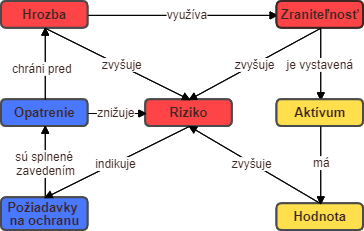
\includegraphics[width=\textwidth,height=6cm,keepaspectratio=true]{assets/risks.png}\end{center}
\caption[Prehľadová schéma riadenia rizík]{Prehľadová schéma riadenia rizík~\cite{RiskManagement}.}\label{obr_1}
\end{figure}

\par Daný problém sa môže vyskytovať aj vo forme zlých právomocí k jednotlivým aktívam. Softvérová firma teda môže mať
navrhnutú výbornú izoláciu medzi jednotlivými projekatmi a zamestnancami. Chybou môže byť aj neprimerané privilégium vo
forme nadmerného prístupu k prostriedku. Príkladom môže byť zamestnanec, ktorý nemá vo firme prístup k dátovému úložisku
a jeho následnému upraveniu. Ak nebol braný do úvahy aj prístup na prehliadanie jednotlivých údajov, takýto zamestnanec
síce nevie dáta zmeniť alebo vymazať, no je schopný prehliadať citlivé údaje a ich obsah zneužiť.

\par Medzi ďalšie problémy patrí takzvaná likvidácia dát. Príkladom môže byť odchod zamestnanca z firmy. Buďe mať stále po roku
prístupy na jeho minulé projekty? Bude mu prístup odobraný po ukončení pracovného pomeru? Prípadne, čo ak na osobnom stretnutí
prezradí prístupové údaje od bývalých projektov? Je možné si tieto údaje útočníkom zapísať a následne sa dostať k prostriedkom?
Čo ak sa samotný zamestnanec bude chcieť po nečakanej výpovedi pomstiť napáchaním škôd? V situácii, kedy zamestnanec nemá
zrušené prístupové údaje, pričom bývalý projekt je nasadený a v praxi využívaný sa jedná o veľmi veľké bezpečnostné riziko.

\par Ak sa jedná o manipuláciu so samotnými citlivými a prístupovými údajmi, tie môžu podliehať, ako bolo už spomínané
neautorizovaným osobám. Medzi najzákladnejšie riziká sú nekryptované, alebo nehašované citlivé dáta uložené v surovej forme
na dátovom úložisku. Príkladom využitia danej zraniteľnosti môže byť heslo používateľa. Správca ani vlastník systému by nemal
vedieť prístupové údaje používateľov v systéme. Tu je možná forma zneužitia takýchto informácií k prístupu do používateľovho
konta. U systémov pracujúcich s finančnými prostriedkami, by mohlo ísť o krádež finančných prostriedkov používateľov vo
vlastný prospech.

\par Prístup k vzdialeným zariadeniam zákazníka firmy by mala mať iba osoba, ktorá má na starosti nasadenie softvérového riešenia.
Keďže sa jedná o veľmi zodpovenú rolu vo firme, možnou hrozbou je zneužitie prístupových údajov odchytením pomocou útoku
MITM~\cite{MITM}, prípadne vyzradením údajov tretej strane podľahnutím phishing útoku~\cite{Phishing}.
Je možné sa chrániť aj proti takýmto hrozbám?

\begin{figure}[H]
\begin{center}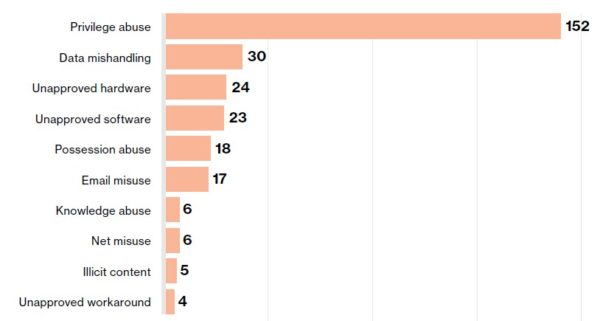
\includegraphics[width=\textwidth,height=6cm,keepaspectratio=true]{assets/priviledge_abuse.jpg}\end{center}
\caption[Najslabšie bezpečnostné miesta v softvérových firmách]{Najslabšie bezpečnostné miesta v softvérových firmách~\cite{WeaknestLink}.}\label{obr_2}
\end{figure}

\par Ako môžme vidieť na obrázku~\ref{obr_2}, najzraniteľnejším miestom v softvérových firmách je zneužitie práv zamestnancov.

\section{Súčasné opatrenia chrániace pred hrozbami}\label{sec:podsekcia-2}

\par Po vymenovaní konkrétnych hrozieb a možných rizík, ktoré z nich vyplívajú je dôležité zistiť formu súčasnývh riešení
protiopatrení, ktoré sú schopné možné riziká odstrániť, prípadne znížiť ich naplnenie. V praxi je nutné finančne predpovedať
náklady firmy vynaložené na opatrenie a finančne predpovedať náklady možného následku po zneužití rizika. Ak je napáchaná
škoda zo zneužitia nižšia, ako dané protiopatrenie na zamedzenie takejto formy útoku, pre softvérovu firmu a jej zákazníkov
je zamedzenie takéhoto typu hrozby z pohľadu manažmentu neoptimálne. Z takýchto, pre firmu nepodstatných rizík je vytvorený
zoznam takzvaných zvyškových rizík, pričom ich znázornenie môžme vidieť na obrázku~\ref{obr_3}.

\begin{figure}[H]
\begin{center}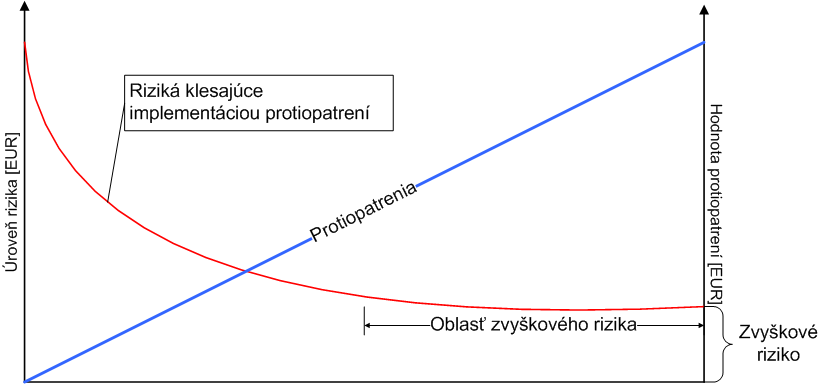
\includegraphics[width=\textwidth,height=6cm,keepaspectratio=true]{assets/zvyskove_riziko.png}\end{center}
\caption[Vizualizácia zvyškových rizík na základe hodnoty protiopatrení]{Vizualizácia zvyškových rizík na základe hodnoty protiopatrení~\cite{RiadenieRizik}.}\label{obr_3}
\end{figure}

\par Priebeh celého procesu riadenia rizík sa vykonáva v nasledovných krokoch. V prvom rade je nutné identifikovať riziko.
Druhým krokom je na základe druhu rizika vhodne stanoviť druh protiopatrenia. Medzi možné spôsoby patria: Zníženie rizika,
Presun rizika, Vyhnutie sa riziku, alebo zachovanie rizika. Po validácii ošetreného rizika vznikajú podproblémy vo forme
zvyškových rizík. Tieto zvyškové riziká sú akceptované vtedy, ak nákladovosť na ich protiopatrenia sú vyššie, ako ich výška
možných škôd. Kontinuálne vykonávanie procesu riadenia rizík je možné znázorniť aj na upravenom Demingovom cykle (tzv. model PDCA)
z bezpečnostnej normy ISO 27001. Vykonávanie podľa daného modelu sa realizuje v štyroch fázach a to: Plánovať – Vykonávať –
Kontrolovať – Pôsobiť. Takýto model je možné prispôsobiť a upraviť pre potreby procesu riadenia rizík podľa obrázka~\ref{obr_3}
nasledovne.

\begin{figure}[H]
\begin{center}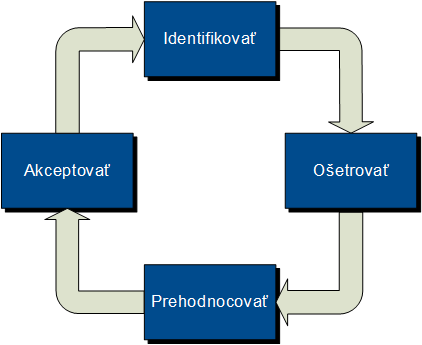
\includegraphics[width=\textwidth,height=6cm,keepaspectratio=true]{assets/pdca.png}\end{center}
\caption[Upravený PDCA model z normy ISO 27001]{Upravený PDCA model z normy ISO 27001~\cite{RiadenieRizik}.}\label{obr_4}
\end{figure}

\par Po stručnom vysvetlení procesu riadenia rizík z pohľadu manažmentu informačnej bezpečnosti je na rade vysvetlenie
jednotlivých hrozieb spomenutých v predchádzajúcej časti práce.

\par Prvou hrozbou bol neautorizovaný prístup k aktívam neoprávnenými
osobami. Daný problém je z veľkej miery ovplivnený vnútornou hierarchiou firmy. Ak firma má v súčasnosti vytvorenú hierarchiu
a každý zamestnanec má svoju špecifickú rolu na danom projekte, nutnosťou pre zamedzenie výskytu rizík vyplívajúcich z
danej hrozby je nasadenie systému autorizácie, ktorý bude jednotlivé roly vo firme validovať, pričom prístup zamietne
tým zamestnancom, ktorých rola nedovoľuje prístup k danému aktívu.

\par Jedným z najrelevantnejších (presne mapujúci danú hierarchiu firmy do systému) autorizačných modelov v súčasnej dobe, je riadenie prístupu na základe rolí (Role Based
Access Control - RBAC) podľa štandardu definovanom v ANSI/INCITS 359–2004~\cite{RBAC}. Daný model patrí k ideológii opatrnej
bezpečnostnej politiky~\cite{OpatrnaBezpecnostnaPolitika}. Podstatou danej ideológie je skutočnosť, že v systéme je zakázané
všetko, čo nie je explicitne povolené. Tým pádom si vieme model RBAC rozdeliť na dve časti. Prvou je zoznam všetkých oprávnení,
ktoré sú v systéme umožnené. Druhou skupinou sú jednotlivé role, ktoré majú podľa ich významu zodpovedajúce oprávnenia.
RBAC implementácia spočíva v štyroch procesoch: Vytvorenie používateľa, vytvorenie role, priradenie role používateľovi,
a priradenie oprávnenia roli. Jedným z problémov nastávajúcich v dynamických softvérových firmách sú výnimky vzhľadom
na určité meniace sa podmienky. Následkom výnimky vznikajú ďalšie role, ktorých počet môže byť časom neudržateľný,
pričom takto zneužité riešenie autorizovaného prístupu má za následok opätovné zvýšenie rizika zneužitia právomocí.
Jedným z možných riešení je vytvorenie dodatočnej tretej časti spočívajúcej vo vzťahu medzi samotným používateľom a
oprávneniami. Takýto vzťah by pre každého používateľa v systéme bol unikátny a nezávislý od jeho role, na rozdieľ od mätúceho
vytvárania rozličných rolí s výnimkami. Ďalšou výhodou takéhoto vzťahu je oddelenie medzi oprávneniami rolí a výnimkovými
oprávneniami pre konkrétnich používateľov.

\par Medzi veĺmi diskutované autorizačné metódy patrí riadenie prístupov na základe atribútov (Attribute-based access
control - ABAC), pričom kĺúčový štandard, z ktorého ABAC vzišiel je XACML~\cite{XACML}. Samotný koncept
sa považuje za autorizačný model "novej generácie". Dôvodom je iný spôsob prístupu k
autorizačnej problematike. Narozdieľ od RBAC udeľovanie prístupu používateľom sa riadi na základe jednotlivých aktív,
inak povedané každej súčasti systému~\cite{ABAC_RBAC_Attributes}. Tento spôsob je veľmi užitočný, práve v spomínaných veľkých korporátnych softvérových
firmách s veľmi výraznou dynamikou riadenia. Pridelenie rolí používateľom teda naďalej nezávisí od ich role, ale od
jednotlivých autorizačných pravidiel vyplívajúcich z namapovaných firemných aktív. Týmto spôsobom je dokonca možné hodnotiť
atribúty subjektov a zdrojov ešte pred ich zavedením do autorizačného systému. Na druhej strane má daný koncept obmedzenie
v konfigurácii, pričom určenie povolení daného používateľa je vzhľadom na návrh metódy veľmi obtiažne. Pre danú bezpečnostnú
problematiku, ktorou sa v práci zaoberáme vznikajú ďalšie nevýhody tohto riešenia a to náročnosť implementácie a bezvýznamnosť danej metódy pre
softvérové firmy menších rozmerov. Na implementáciu daného konceptu je taktiež nutný podrobný návrh firemnej politiky~\cite{RBAC_ABAC_Encryption}.

\par Druhou hrozbou, ktorá so sebou prinášala veľký počet rizík bola otázka likvidácie dát. Jednoduchým teoretickým
riešením je všetky dáta a účty, ktoré už nie sú potrebné vymazať. Realita vo firmách je žial oveľa zložitejšia. Ak zamestnanec
z firmy odíde, neostane po ňom vo väčšine malých firiem iba jedno konto. Tieto kontá a prístupové údaje bude nutné všetky vyhľadať,
pričom sa vyskytujú na rôznych zariadeniach, službách technológiach a podobne. Preto musí byť touto pracnou úlohou poverený
zamestnanec z firmy, ktorému môže celý proces trvať niekoľko minút až hodín. Takýto spôsob likvidácie dát je veľmi časovo náročný
a hľavne obsahuje veľké riziko omylu a prehliadnutia niektorých z účtov. Dané riziko nemusí explicitne vzísť iba z odchodu
zamestnanca z firmy. Zamestnancom sa počas pôsobenia v praxi môže meniť ich rola, projekty na ktorých pracujú, môže sa odstrániť
služba, ku ktorej musí mať prihlasovacie údaje a podobne. Všetky tieto scenáre by mali byť riešené bezpečným, jednoduchým a
centralizovaným spôsobom.

\par Jedným z riešení, ako sa vyhnúť daným rizikám je vytvorenie centrálnej autentifikácie zamestnancov. Tým by sa
zamedzilo udržiavaniu ich prihlasovacích údajov na viacerých miestach. Jednou z možností je autentifikácia pomocou ľahkého
protokolu prístupu k adresáru (Lightweight Directory Access Protocol - LDAP)~\cite{LDAP}. Cieľom je vytvorenie
servera, ktorý bude spravovať firemné prihlasovacie údaje jednotlivých zamestnancov, pričom jednotlivé služby softvérovej
firmy, ku ktorým je nutná autentifikácia budú podporovať autentifikáciu pomocou LDAP protokolu~\cite{LDAP_AUTH}. Takéto riešenie by malo
za následok správu všetkých kont zamestnancov na jednom mieste. Ak by nastali popísané rizikové situácie, likvidácia dát je umožnená
z jednoho centralizovaného bodu. Priebeh autentifikácie na firemné aplikácie a služby by prebiehal podľa schémy na
obrázku~\ref{obr_5}.

\begin{figure}[H]
\begin{center}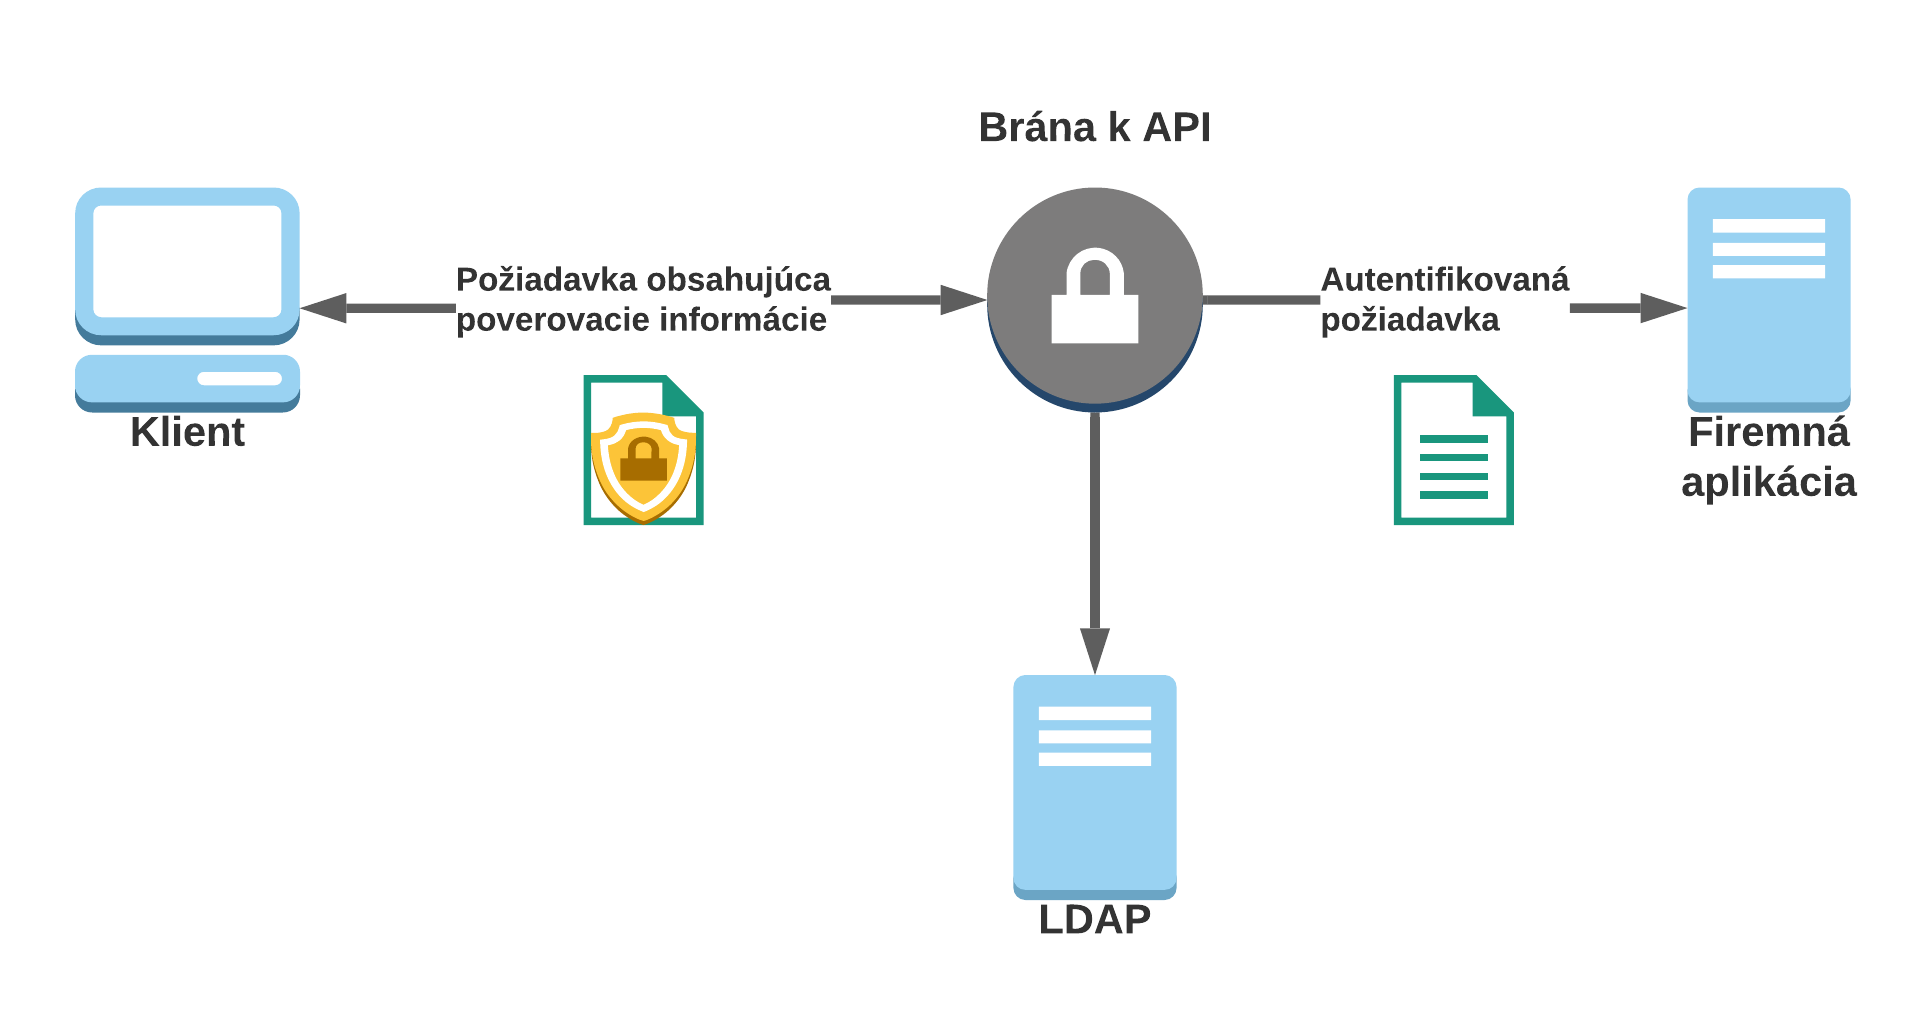
\includegraphics[width=\textwidth,height=6cm,keepaspectratio=true]{assets/ldap_schema.png}\end{center}
\caption[Schéma prihlasovania podľa protokolu LDAP]{Schéma prihlasovania podľa protokolu LDAP}\label{obr_5}
\end{figure}

\par Treťou hrozbou bol prístup k dátam na dátovom úložisku. Je možné dôverovať osobe s autorizáciou prehliadnia dát s
citlivými informáciami ako napríklad heslá, čísla kariet, prístupové adresy a podobne? Na danú otázku existuje odpoveď
vo forme modelu CIA, známeho aj ako model rozvoja bezpečnostnej politiky~\cite{CIA}. Skratka CIA hovorí o troch dôležitých bezpečnostných
pilieroch manipulácie s dátami. Prvým z nich dôvernosť (Confidentality), ktorý hovorí o neschopnosti zistenia obsahu
dôverných informácíí ktorýmkoľvek používateľom. Ako chceme dôverné informácie ochrániť pred všetkými zamestnancami,
aj tými, ktorí majú k dátovému úložisku nutnú autorizáciu? Bezpečnými spôsobmi ochrany informácií sú enkrypcia a hašovanie.
Enkrypcia je v skratke obojsmerná funkcia. Tým pádom slúži na anonymizovanie statických dát ako napríklad informácie umožňujúce
identifikáciu osôb~\cite{Encryption}. Konkrétne sa môže jednať o dáta typu: Číslo vodičského preukazu, číslo občianskeho preukazu a podobne.
Na druhej strane hašovacia funkcia je jednosmerná. Inak povedané, funkcia nemá možnosť spätného "odhašovania" informácie~\cite{Hashing}.
Bezpečným prvkom, ktorý je k hašovaniu možné pridať je takzvaný "salt", ktorý danú hašovaciu funkciu zamieša špecifickým
reťazcom znakov. Hašovacia funkcia sa používa pri druhoch informácií, ktoré sú posielané medzi dvomi sieťovými bodmi. Napríklad
môže ísť o heslo, ktorého reálnu hodnotu nikdy na strane zariadenia ktoré ho uchováva nemusíme vedieť. Stačí, ak sa rovnaký
spôsob hašovania hesla použije na strane zariadenia vyžadujúceho autentifikáciu. Pri procese autentifikácie sa oba haše
porovnajú a ak sa rovnajú, heslá sa zhodujú. Výsledkom hašovacej funkcie je fixne dlhý reťazec znakov. Napríklad pri texte
dlhom 250 znakov môže byť výsledný haš dlhý 32 znakov. Preto dôležitým atribútom hašovacích funkcií je ich matematicky
veľmi nízka pravdepodobnosť na vytvorenie dvoch rovnakých výstupných reťazcov pri rozdielnych vstupoch. Druhým pilierom modelu
CIA je integrita (Integrity), ktorá hovorí o konzistencii informácií na dátovom úložisku. Ak by došlo k ich modifikácii, vlastník
daných informácií musí byť informovaný o ich zmene. Táto skutočnosť vie ochrániť vlastníkov údajov pred ich nežiadúcou
zmenou, ktorá môže byť spôsobená neautorizovaným prístupom. Posledným pilierom modelu CIA je dostupnosť (Availability).
K skutočnej forme informácií môže mať prístup iba ich vlastník a to v čitateľnej a konečnej podobe. To napríklad znamená,
že pred zobrazením používateľovho rodného čísla musí byť táto enkryptovaná dôverná informácia spätne dekryptovaná do
originálnej podoby.

\par Posledný spomínaný problém nesie so sebou výskyt rizík v podobe získania prístupových údajov, či už sa jedná o autentifikáciu
do firemného systému, alebo dáta potrebné na nasadenie finálneho softvérového produktu ku koncovým zariadeniam zákazníkov.
V oboch prípadoch, ako bolo už spomenuté ide o veľmi vážne bezpečnostné riziká, keďže sa taktiež priamo týkajú zákazníkov
softvérovej firmy. Pre šifrovaný spôsob komunikácie je potrebné implementovať komunikačné protokoly v súlade s bezpečnostnými
požiadavkami. Komunikácia medzi vzdialeným webovým firemným serverom a zamestnancom by hohla prebiehať cez zabezpečený protokol
HTTPS (Hypertext transfer protocol secure)~\cite{HTTPS}, kde by boli jednotlivé autentifikačné dáta na transportnej vrstve
šifrované bezpečnostným protokolom TLS (Transport Layer Security)~\cite{TLS}. Samotný spôsob autentifikácie by mohol byť
uskutočnený podľa formátu JWT (JSON Web Token) spolu s využitím autentifikačného protokolu OAUTH(2.0) (Open standard for
access delegation)~\cite{JWT}. Keďže prístup k firemným zdrojom je veľmi diskrétny, z bezpečnostného hľadiska je odporúčané
použitie dvojfaktorovej autentifikácie~\cite{DvojfaktorovaAutentifikacia}, ktorej priebeh môžme vidieť na obrázku~\ref{obr_6}.
Dvojfaktorová autentifikácia nepodlieha útokom hrubou silou a taktiež po získaní prístupových dát napríklad odchytením,
alebo inou formou útoku nepodlieha ich zneužitu z dôvodu veľmi frekventovane meniaceho sa unikátneho verifikačného kódu.
Pokiaľ sa jedná o komunikáciu medzi koncovými zariadeniami zákazníkov, tú je možné zabezpečiť protokolom SFTP (SSH File
Transfer Protocol)~\cite{SFTP}, ktorý umožňuje posielanie súborov cez protokol SSH (Secure Shell)~\cite{SSH}, slúžiaci
na bezpečné vykonávanie príkazov na vzdialených zariadeniach.

\begin{figure}[H]
\begin{center}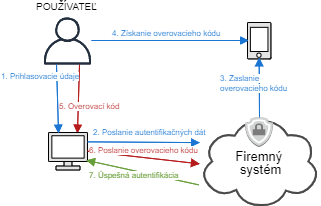
\includegraphics[width=\textwidth,height=6cm,keepaspectratio=true]{assets/auth.png}\end{center}
\caption[Schéma dvojfaktorovej autentifikácie]{Schéma dvojfaktorovej autentifikácie}\label{obr_6}
\end{figure}

\section{Zhodnotenie}\label{sec:podsekcia-3}

\par Z analýzy vyplíva, že jednotlivé problémy spojené s bezpečnostnými rizikami sú v súčastnosti riešiteľné veľkým počtom
rôznych spôsobov protiopatrení. Taktiež existujú presne špecifikované postupy a normy, ktoré je dôležité dodržovať
softvérovými firmami pre zlepšenie ich informačnej bezpečnosti. Otázkou ostáva, z akého dôvodu naďalej väčšina malých
softvérových firiem odkladá, alebo úmyselne prehliada jednotlivé bezpečnostné hrozby. V prvom rade je dôležité si uvedomiť,
že firmy sú schopné jednotlivé bezpečnostné opatrenia vyriešiť, no z dôvodu prekážok, v podobe časových a finančných
prostriedkov im vo väčšine prípadov takáto možnosť riešenia nie je umožnená~\cite{CompanySecurity}. Príkladom môže byť nízky počet zamestnancov,
ktorý sú potrebný na jednotlivých špecializovaných úlohách  pridelených k projektom. Prevelením jednoho zamestnanca z
projektu s cieľom riešenia firemnej bezpečnosti, môže mať za následok rapídne zníženie produktivity na určitých častiach práce. Ďalším reálnym
problémom je financovanie časovo náročných bezpečnostných opatrení, ktorých implementácia je financovaná priamo z firemného
rozpočtu. Jedným z finančne a časovo nenáročných riešení pre softvérové firmy pramení z idei spojenia všetkých analyzovaných
bezpečnostných opatrení do jednoho celku, v podobe informačného bezpečnostného systému. Takýto systém by obsahoval všetky
bezpečnostné aspekty protiopatrení, pričom jeho návrh a implementácia by sa musela prioritne riadiť podľa kritérií vysokej
bezpečnosti, modularity a rozšíriteľnosti. Dôvodom je použitie implementovaného bezpečnostného riešenia v praxi jednotlivými
firmami ako produktu tretej strany, pričom firmy by mohli podľa ich potrieb jednotlivé časti systému ľahko upraviť, prípadne
doplniť o nové bezpečnostné prvky.

\chapter{Návrh}\label{ch:návrh}

\section{Demonštrácia riešenia}\label{sec:demonstracia-riesenia}

\begin{figure}[H]
\begin{center}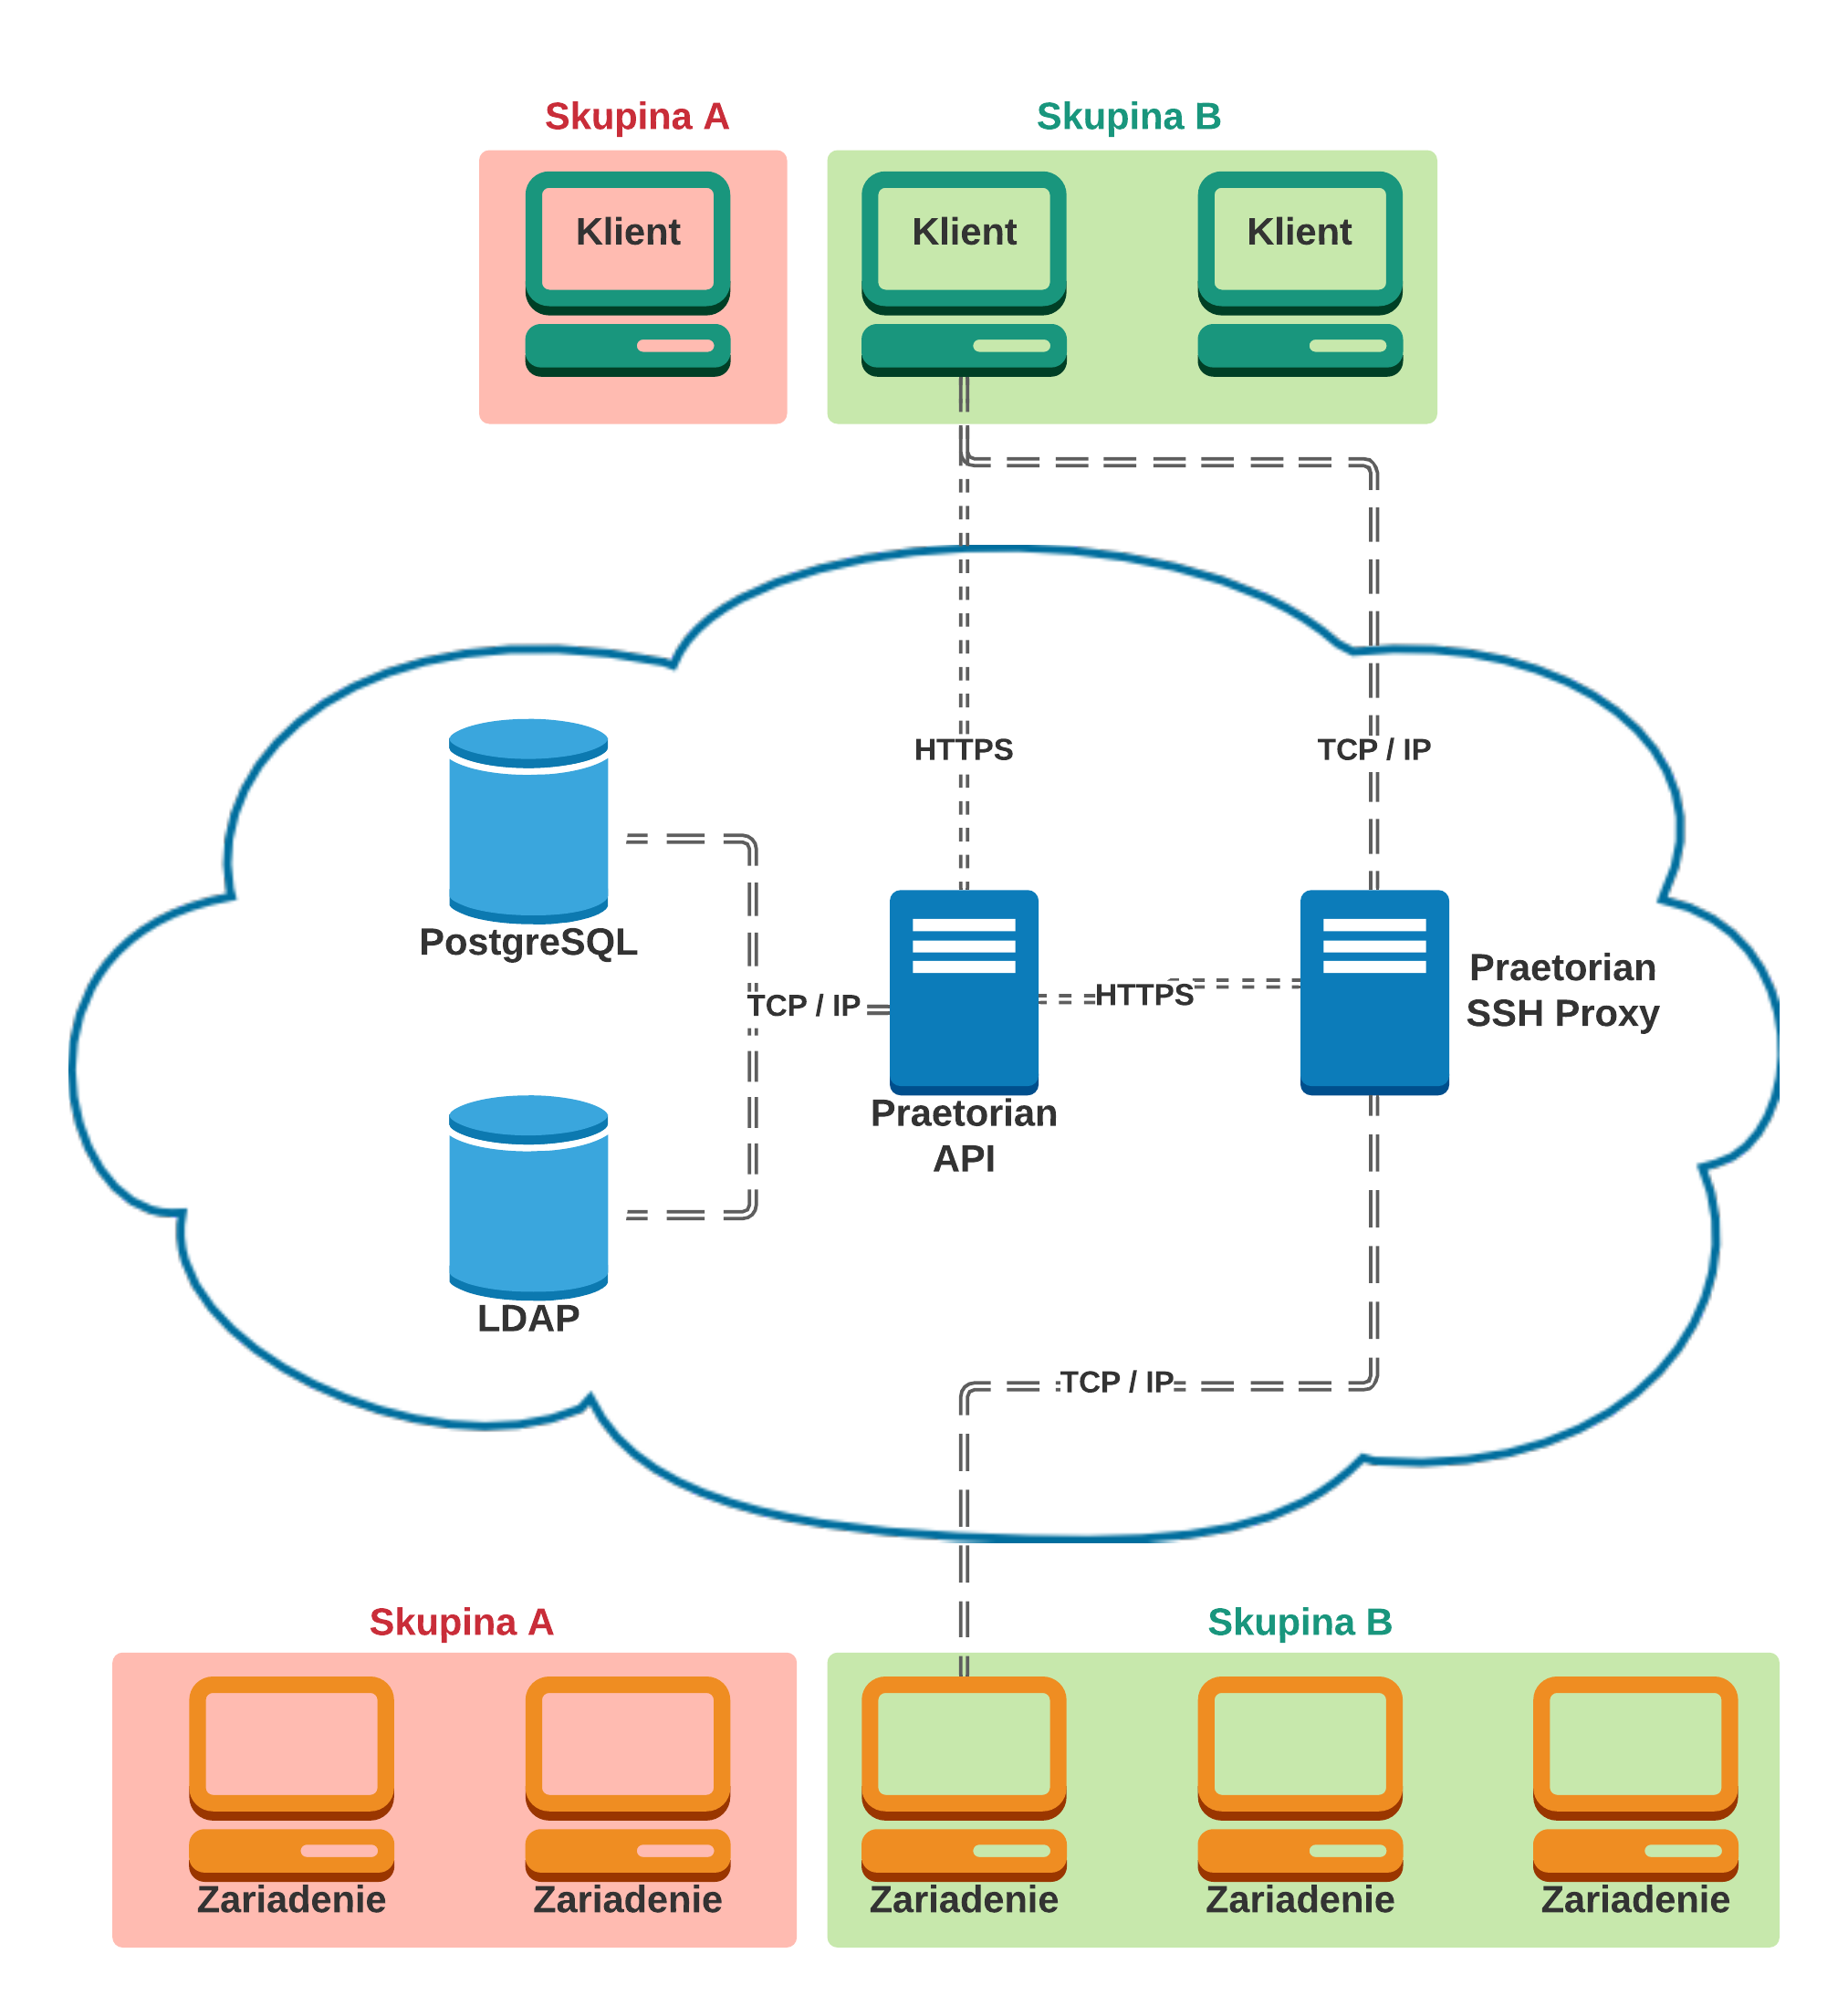
\includegraphics[width=\textwidth,height=12cm,keepaspectratio=true]{assets/demonstracia_riesenia.png}\end{center}
\caption[Demonštrácia riešenia]{Demonštrácia riešenia}\label{fig:obr_8}
\end{figure}

\section{Diagram komponentov}\label{sec:diagram-komponentov}

\begin{figure}[H]
\begin{center}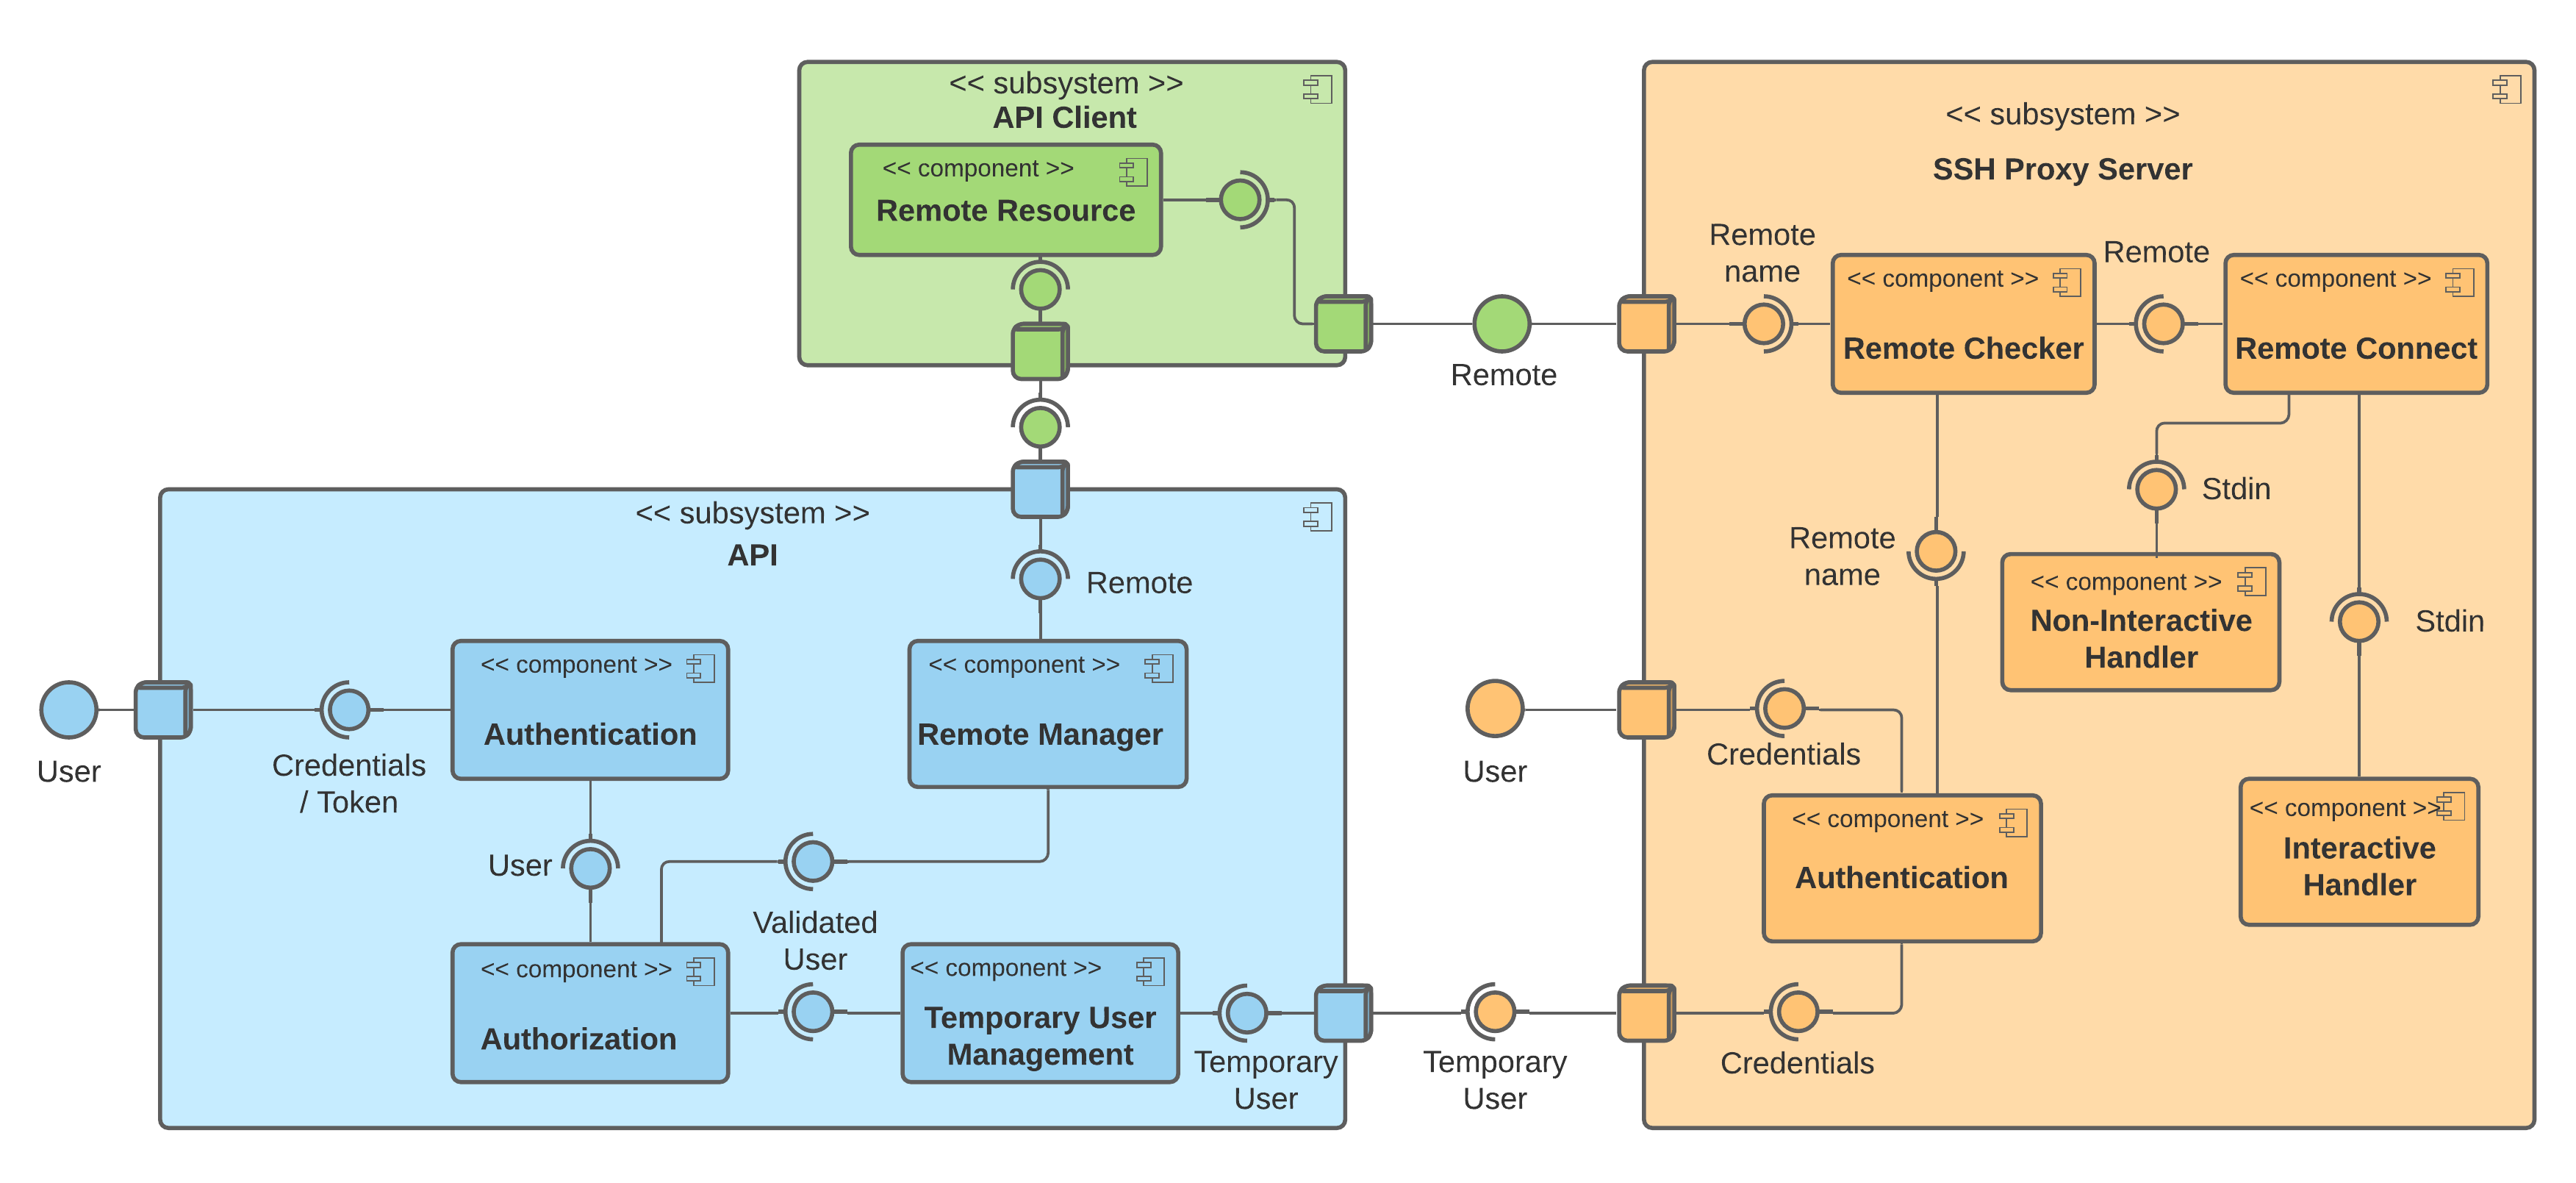
\includegraphics[width=\textwidth,height=8cm,keepaspectratio=true]{assets/diagram_komponentov.png}\end{center}
\caption[Diagram komponentov]{Diagram komponentov}\label{fig:obr_9}
\end{figure}

\section{Sekvenčné diagramy}\label{sec:sekvencne-diagramy}

\subsection{Autentifikácia}\label{subsec:sek-autentifikacia}

\begin{figure}[H]
\begin{center}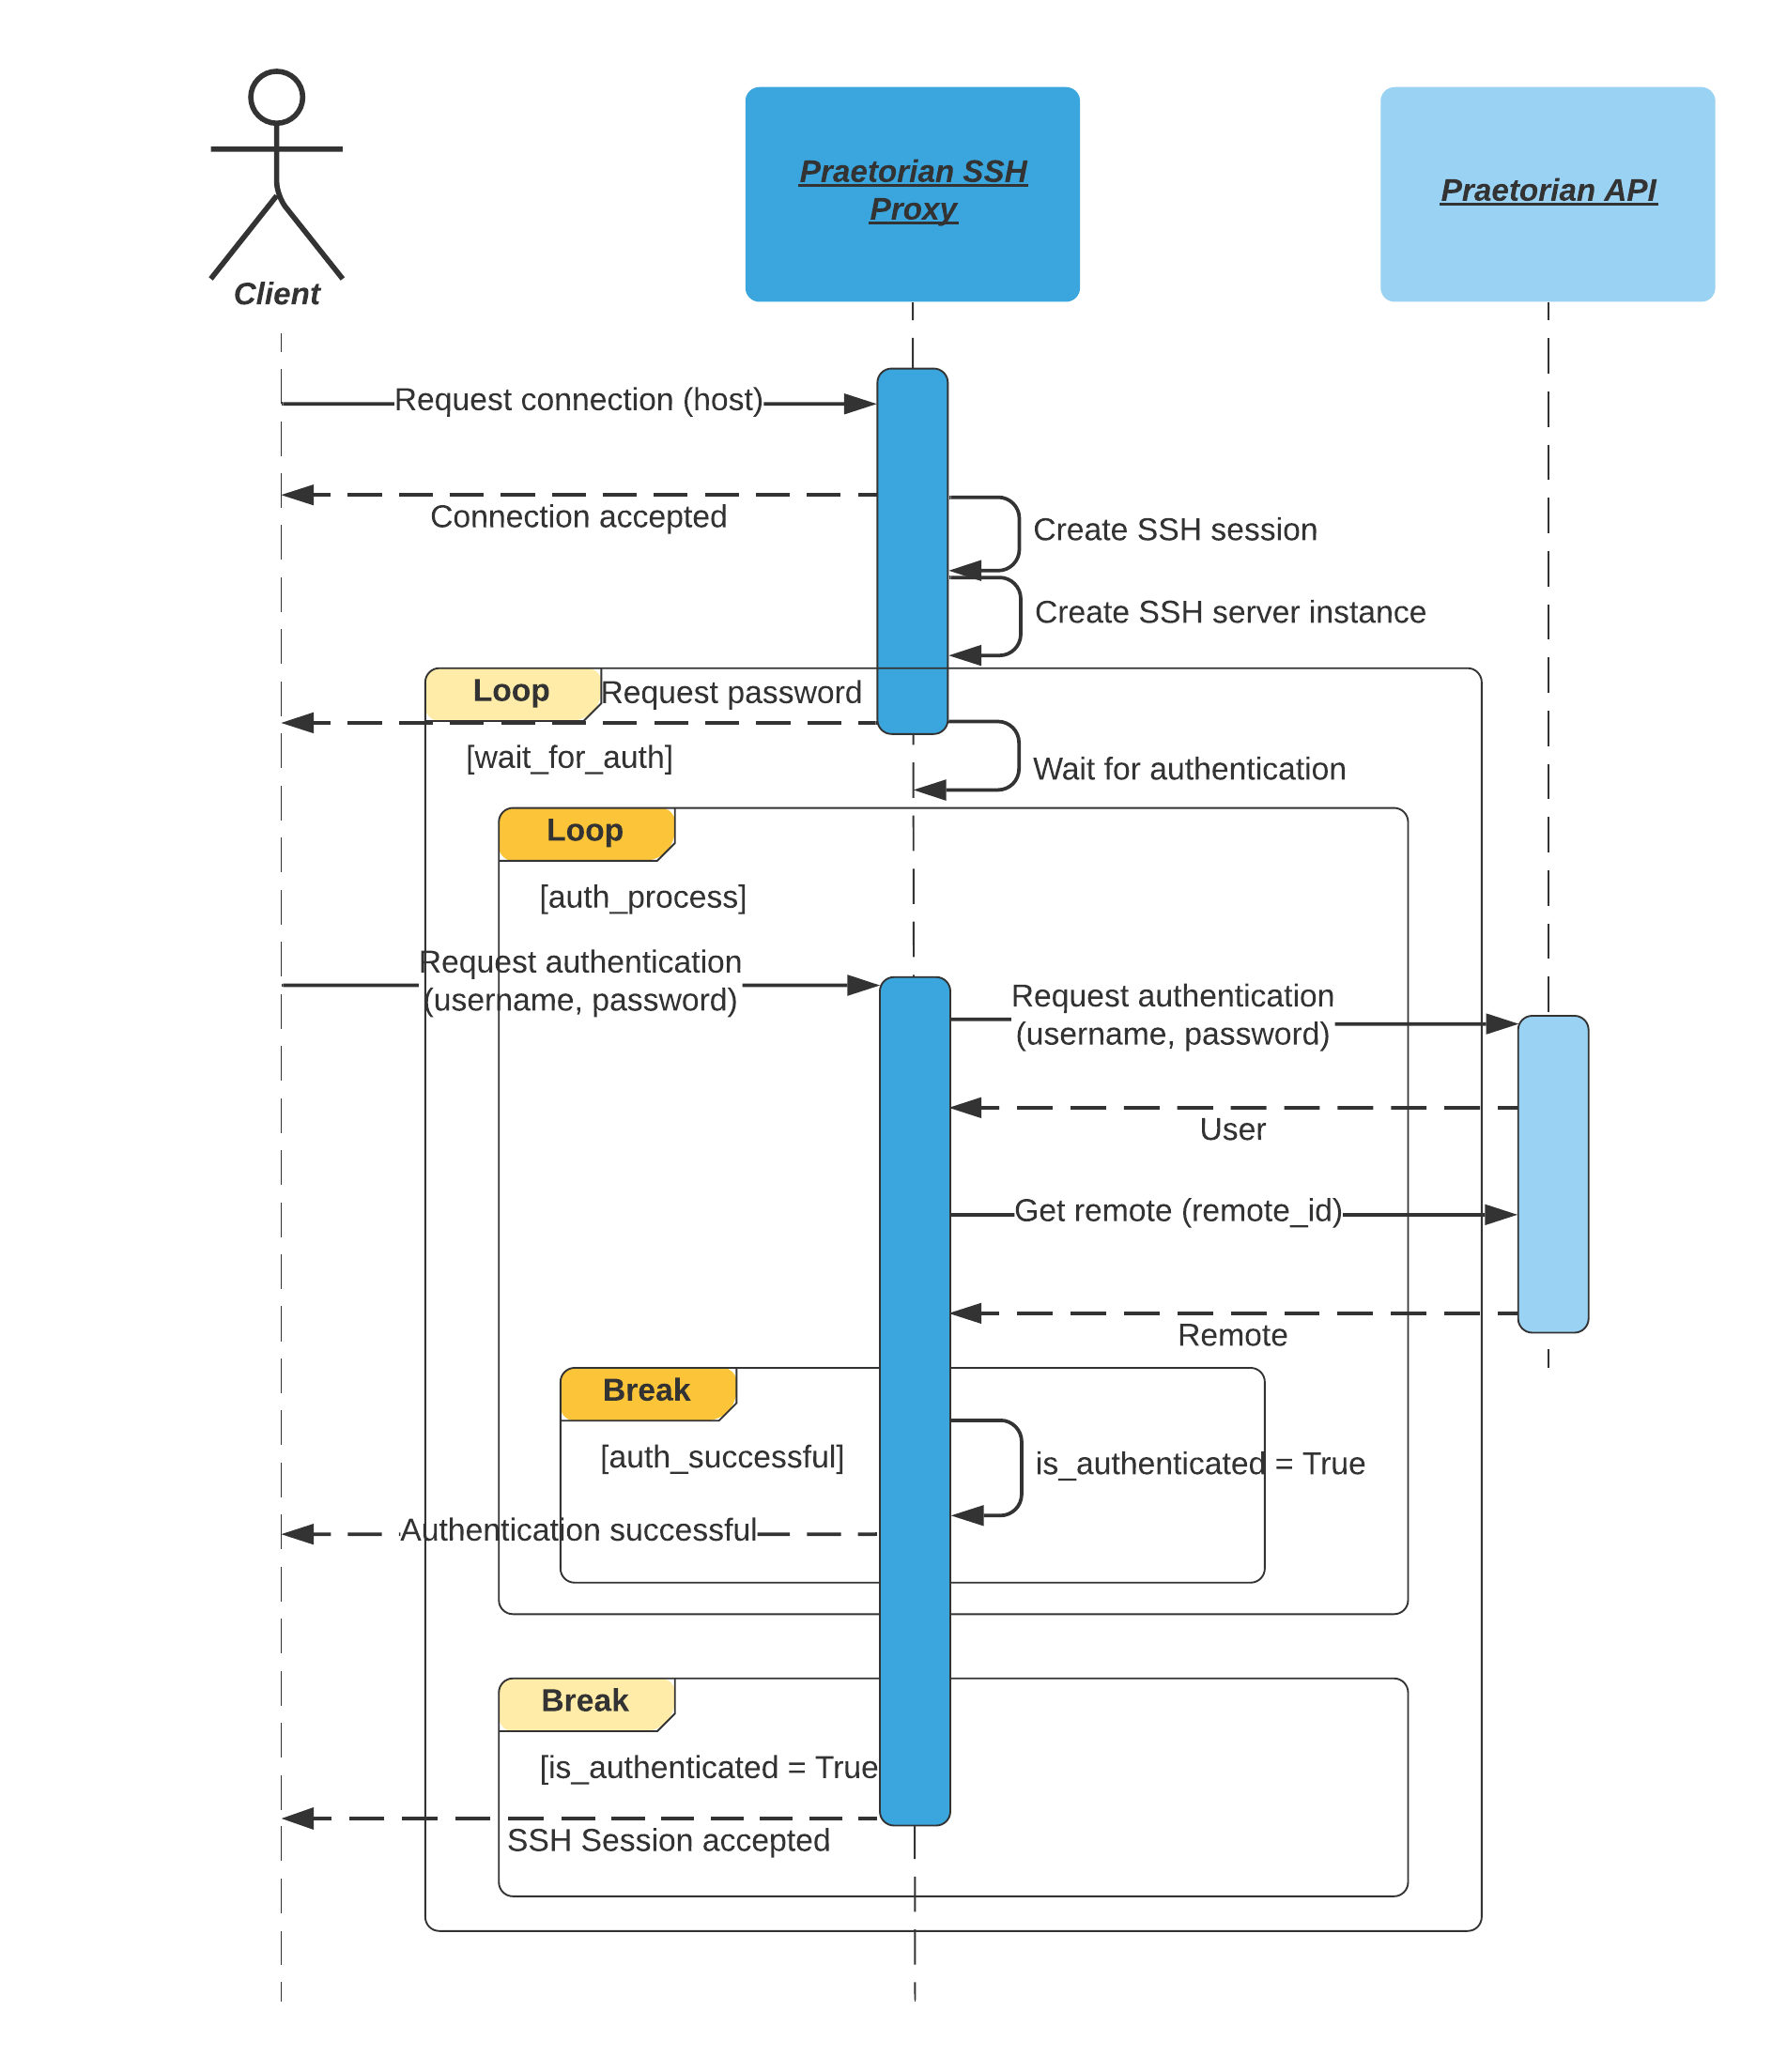
\includegraphics[width=\textwidth,height=12cm,keepaspectratio=true]{assets/sequence_diagram_auth.png}\end{center}
\caption[Autentifikácia]{Autentifikácia}\label{fig:obr_10}
\end{figure}

\subsection{Interaktívne prostredie}\label{subsec:interkativne-prostredie}

\begin{figure}[H]
\begin{center}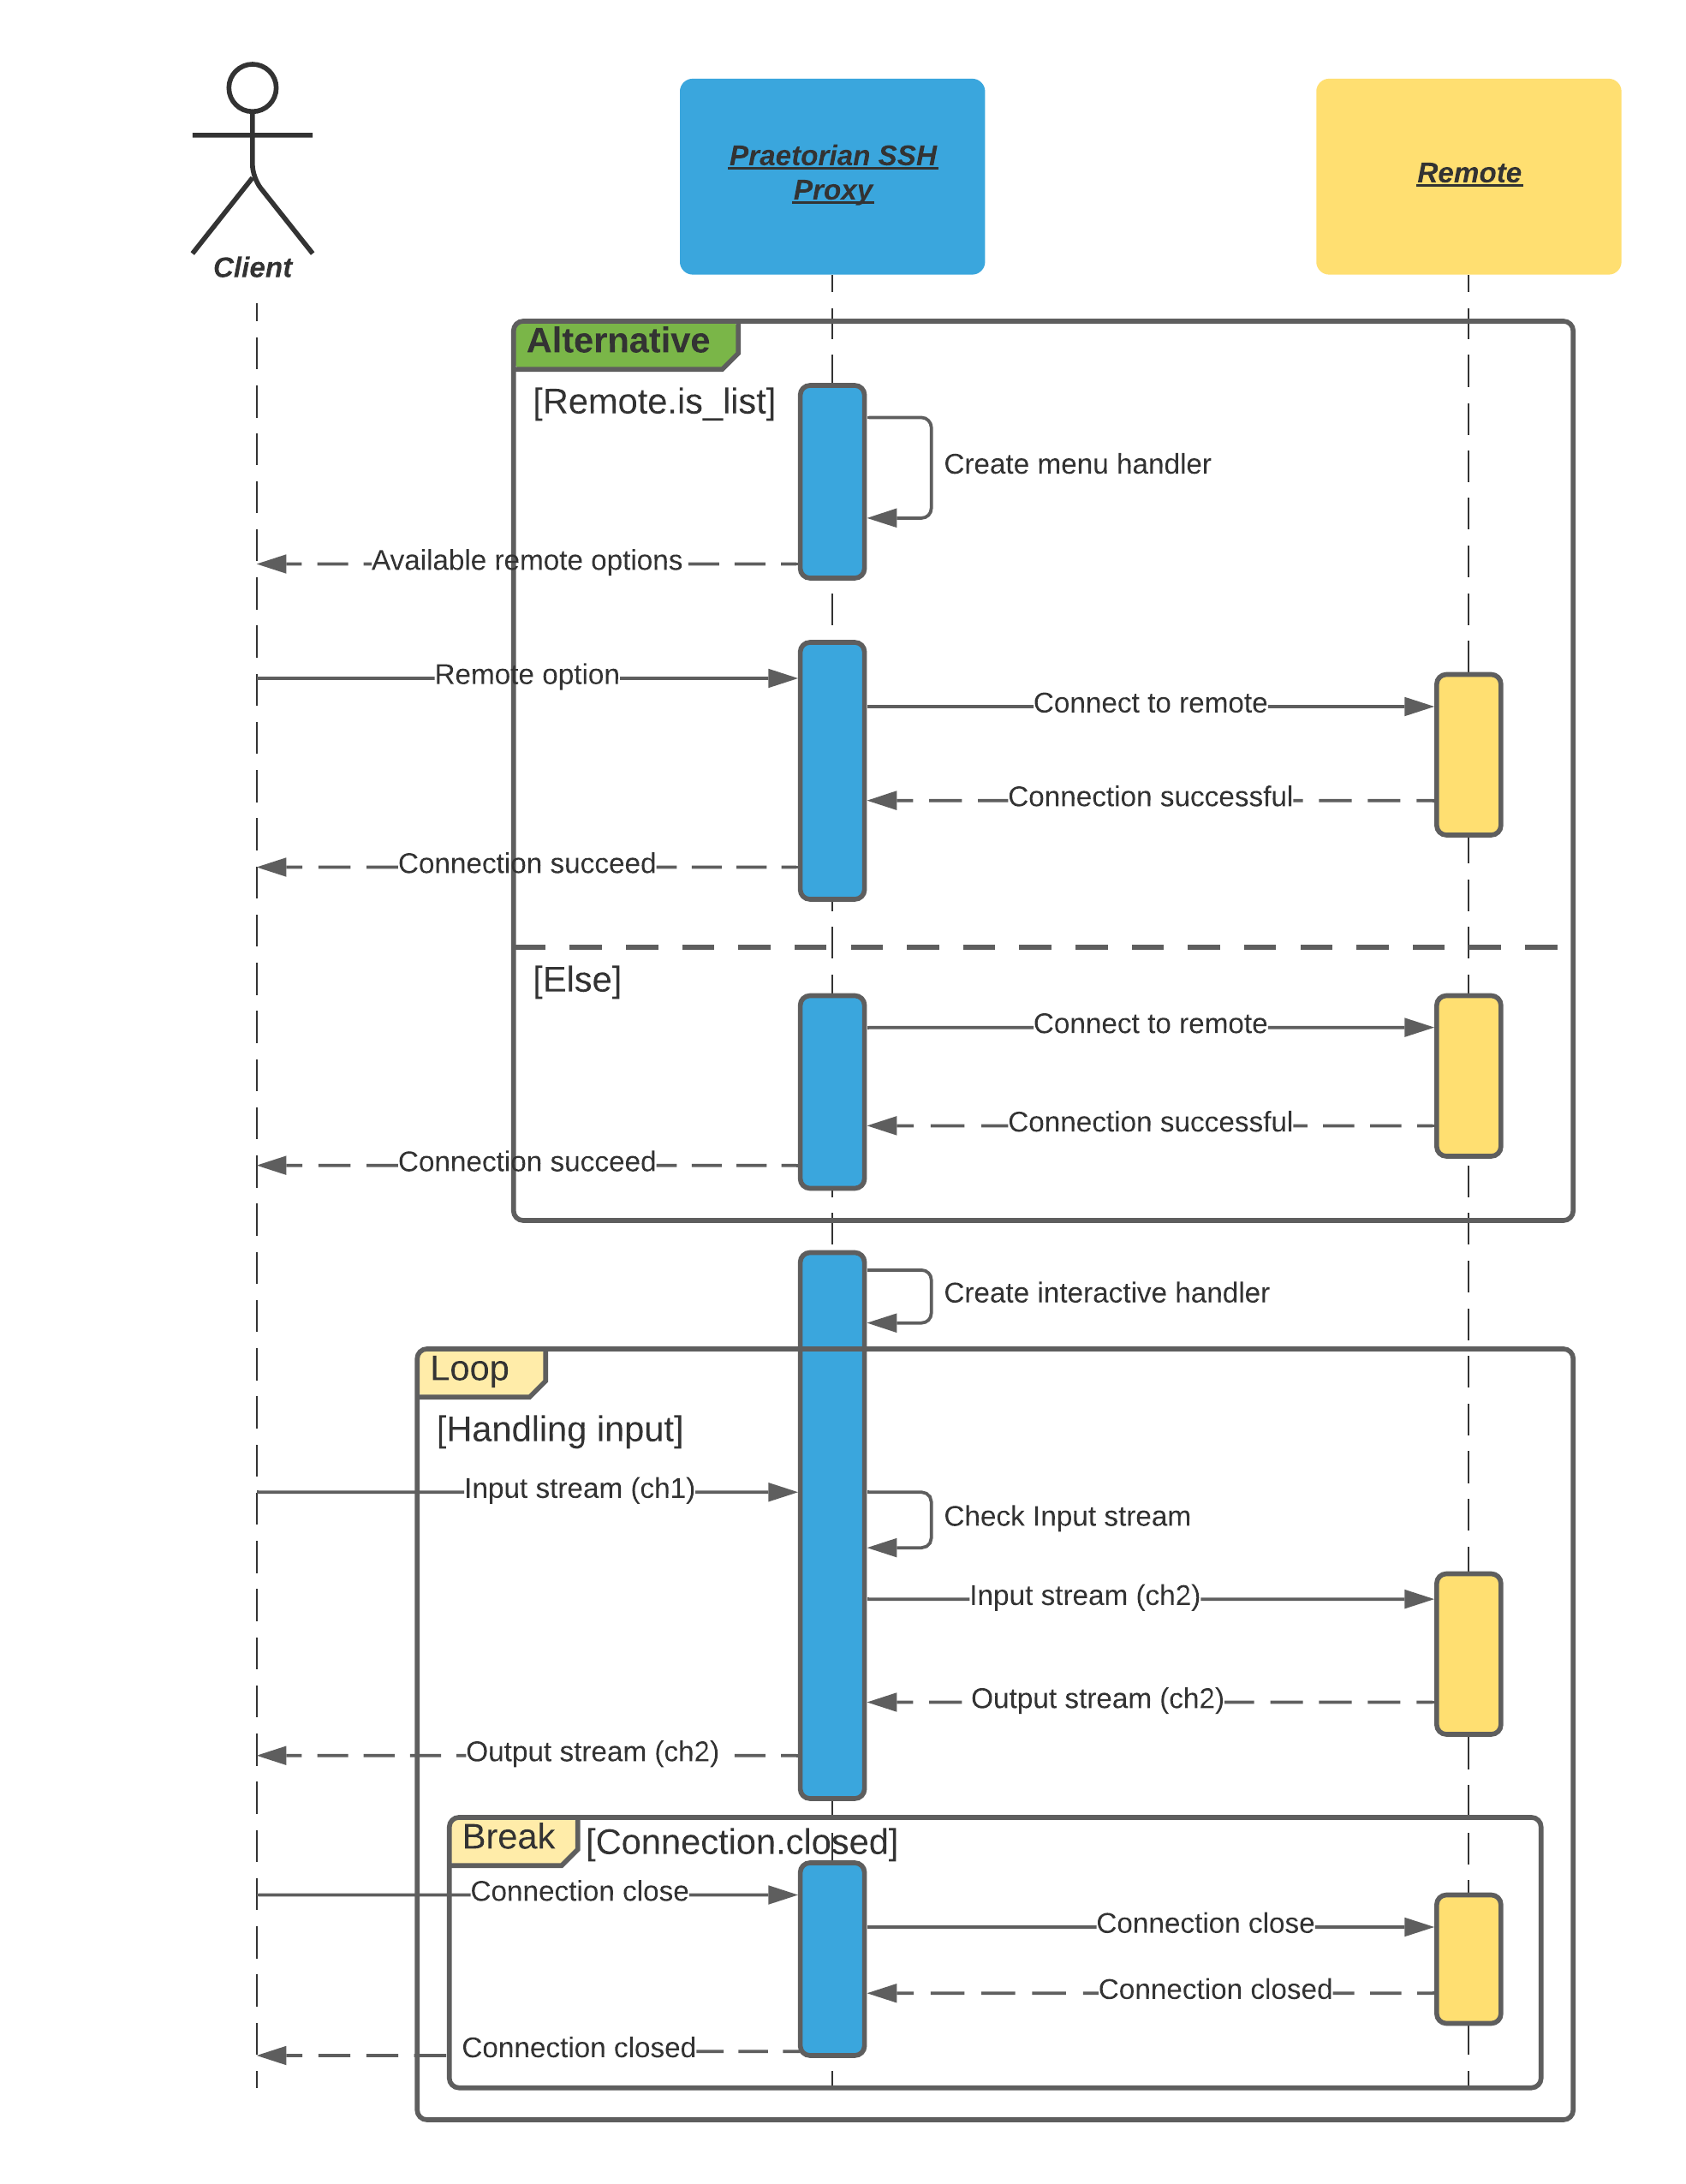
\includegraphics[width=\textwidth,height=12cm,keepaspectratio=true]{assets/sequence_diagram_interactive.png}\end{center}
\caption[Interaktívne prostredie]{Interaktívne prostredie}\label{fig:obr_11}
\end{figure}


\subsection{Neinteraktívne prostredie}\label{subsec:neinterkativne-prostredie}

\begin{figure}[H]
\begin{center}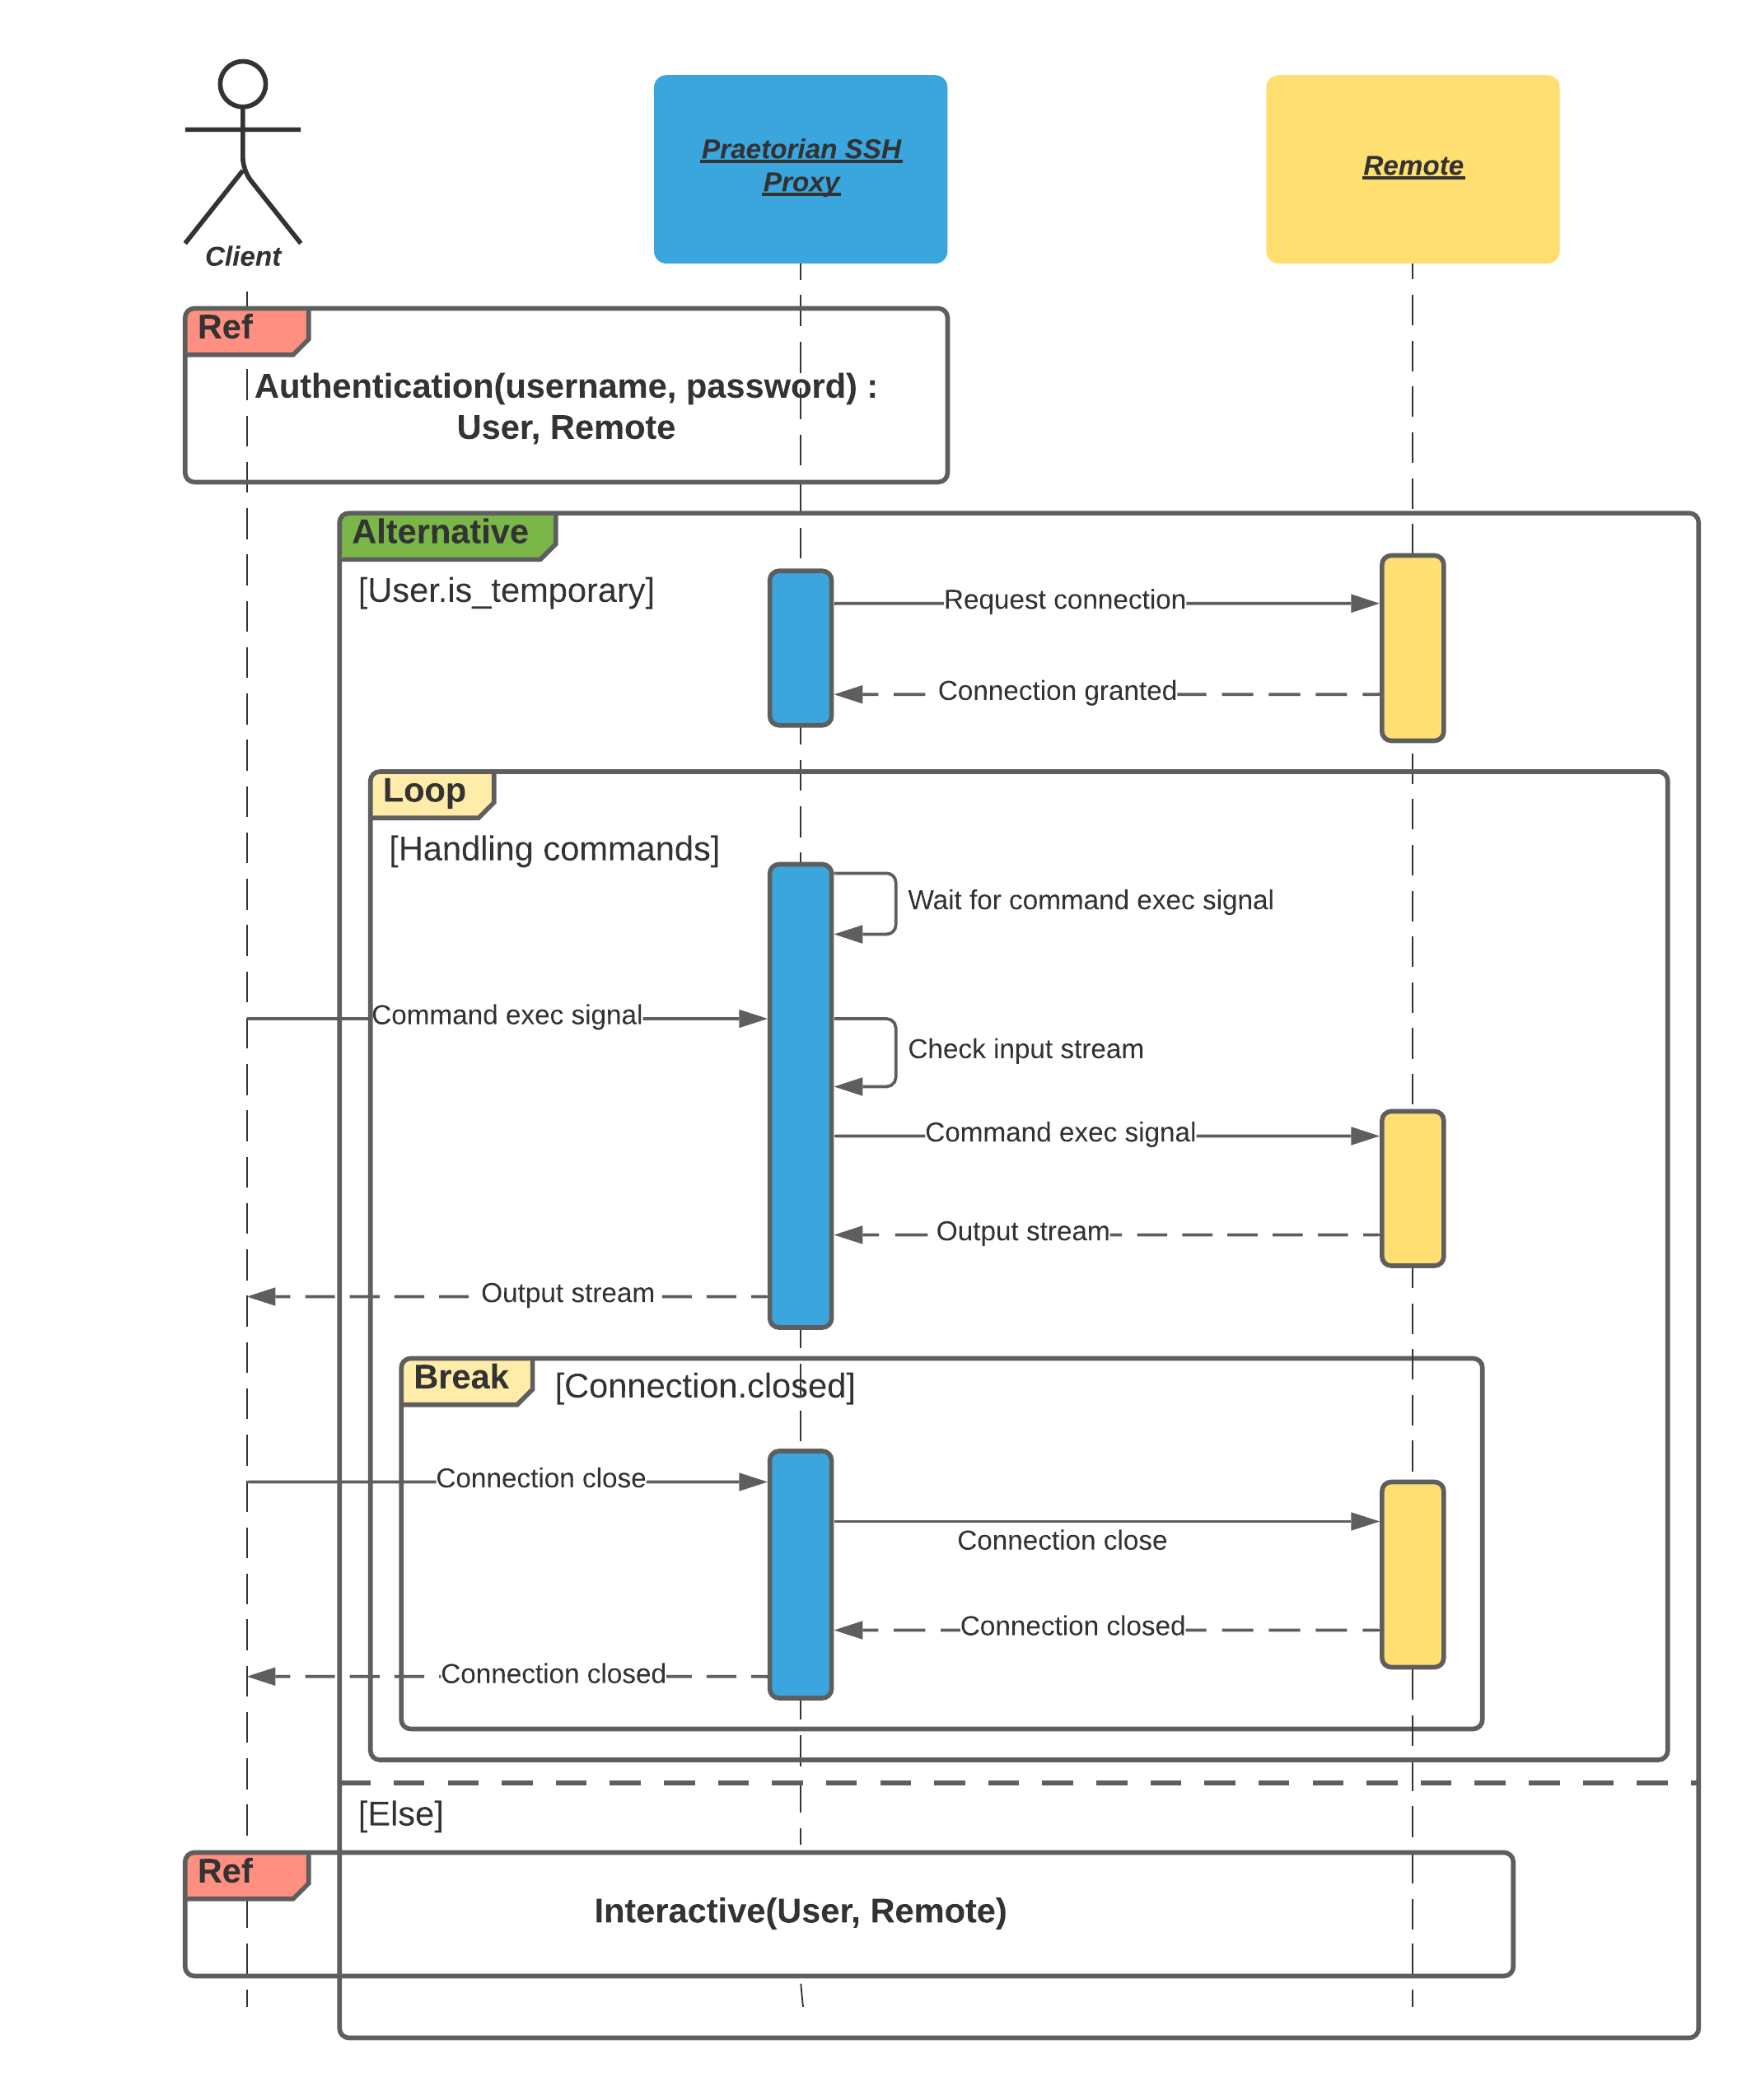
\includegraphics[width=\textwidth,height=12cm,keepaspectratio=true]{assets/sequence_diagram_non_interactive.png}\end{center}
\caption[Neinteraktívne prostredie]{Neinteraktívne prostredie}\label{fig:obr_12}
\end{figure}

\chapter{Návrh riešenia}\label{ch:návrh}

\section{Demonštrácia riešenia}\label{sec:demonstracia-riesenia}

Prvým krokom pri návrhu riešenia, bolo z pohľadu informačnej bezpečnosti presne zadefinovať a rozanalyzovať hlavné prípady
použitia.
Medzi hlavné prípady použitia, ktoré boli zadefinované s cieľom formovania myšlienky boli napríklad: Konfigurovateľná správa
vnútorno-firemnej bezpečnostnej politiky v nami navrhnutej webovej aplikácii, prísne zadefinovaná hierarchia a vzťah medzi objektami,
riadenie celého procesu nasadenia, alternatívne možnosti prístupov s bezpečným dohľadom nad všetkými operáciami a komunikačnými správami.
Medzi najhlavnejšie kritéria, ktorými bol riadený celý proces návrhu boli bezpečnosť a modularita riešenia.
Preto bolo zadefinovaných päť majoritných entít: webové api, ssh proxy server, api klient, používateľ a koncové zariadenie.
Tieto vymenované entity medzi sebou komunikujú a interagujú v presne zadefinovanej a zabezpečenej schéme, ktorú môžme vidieť
v nasledujúcom grafickom náhľade riešenia~\ref{fig:obr_8}.

\begin{figure}[H]
\begin{center}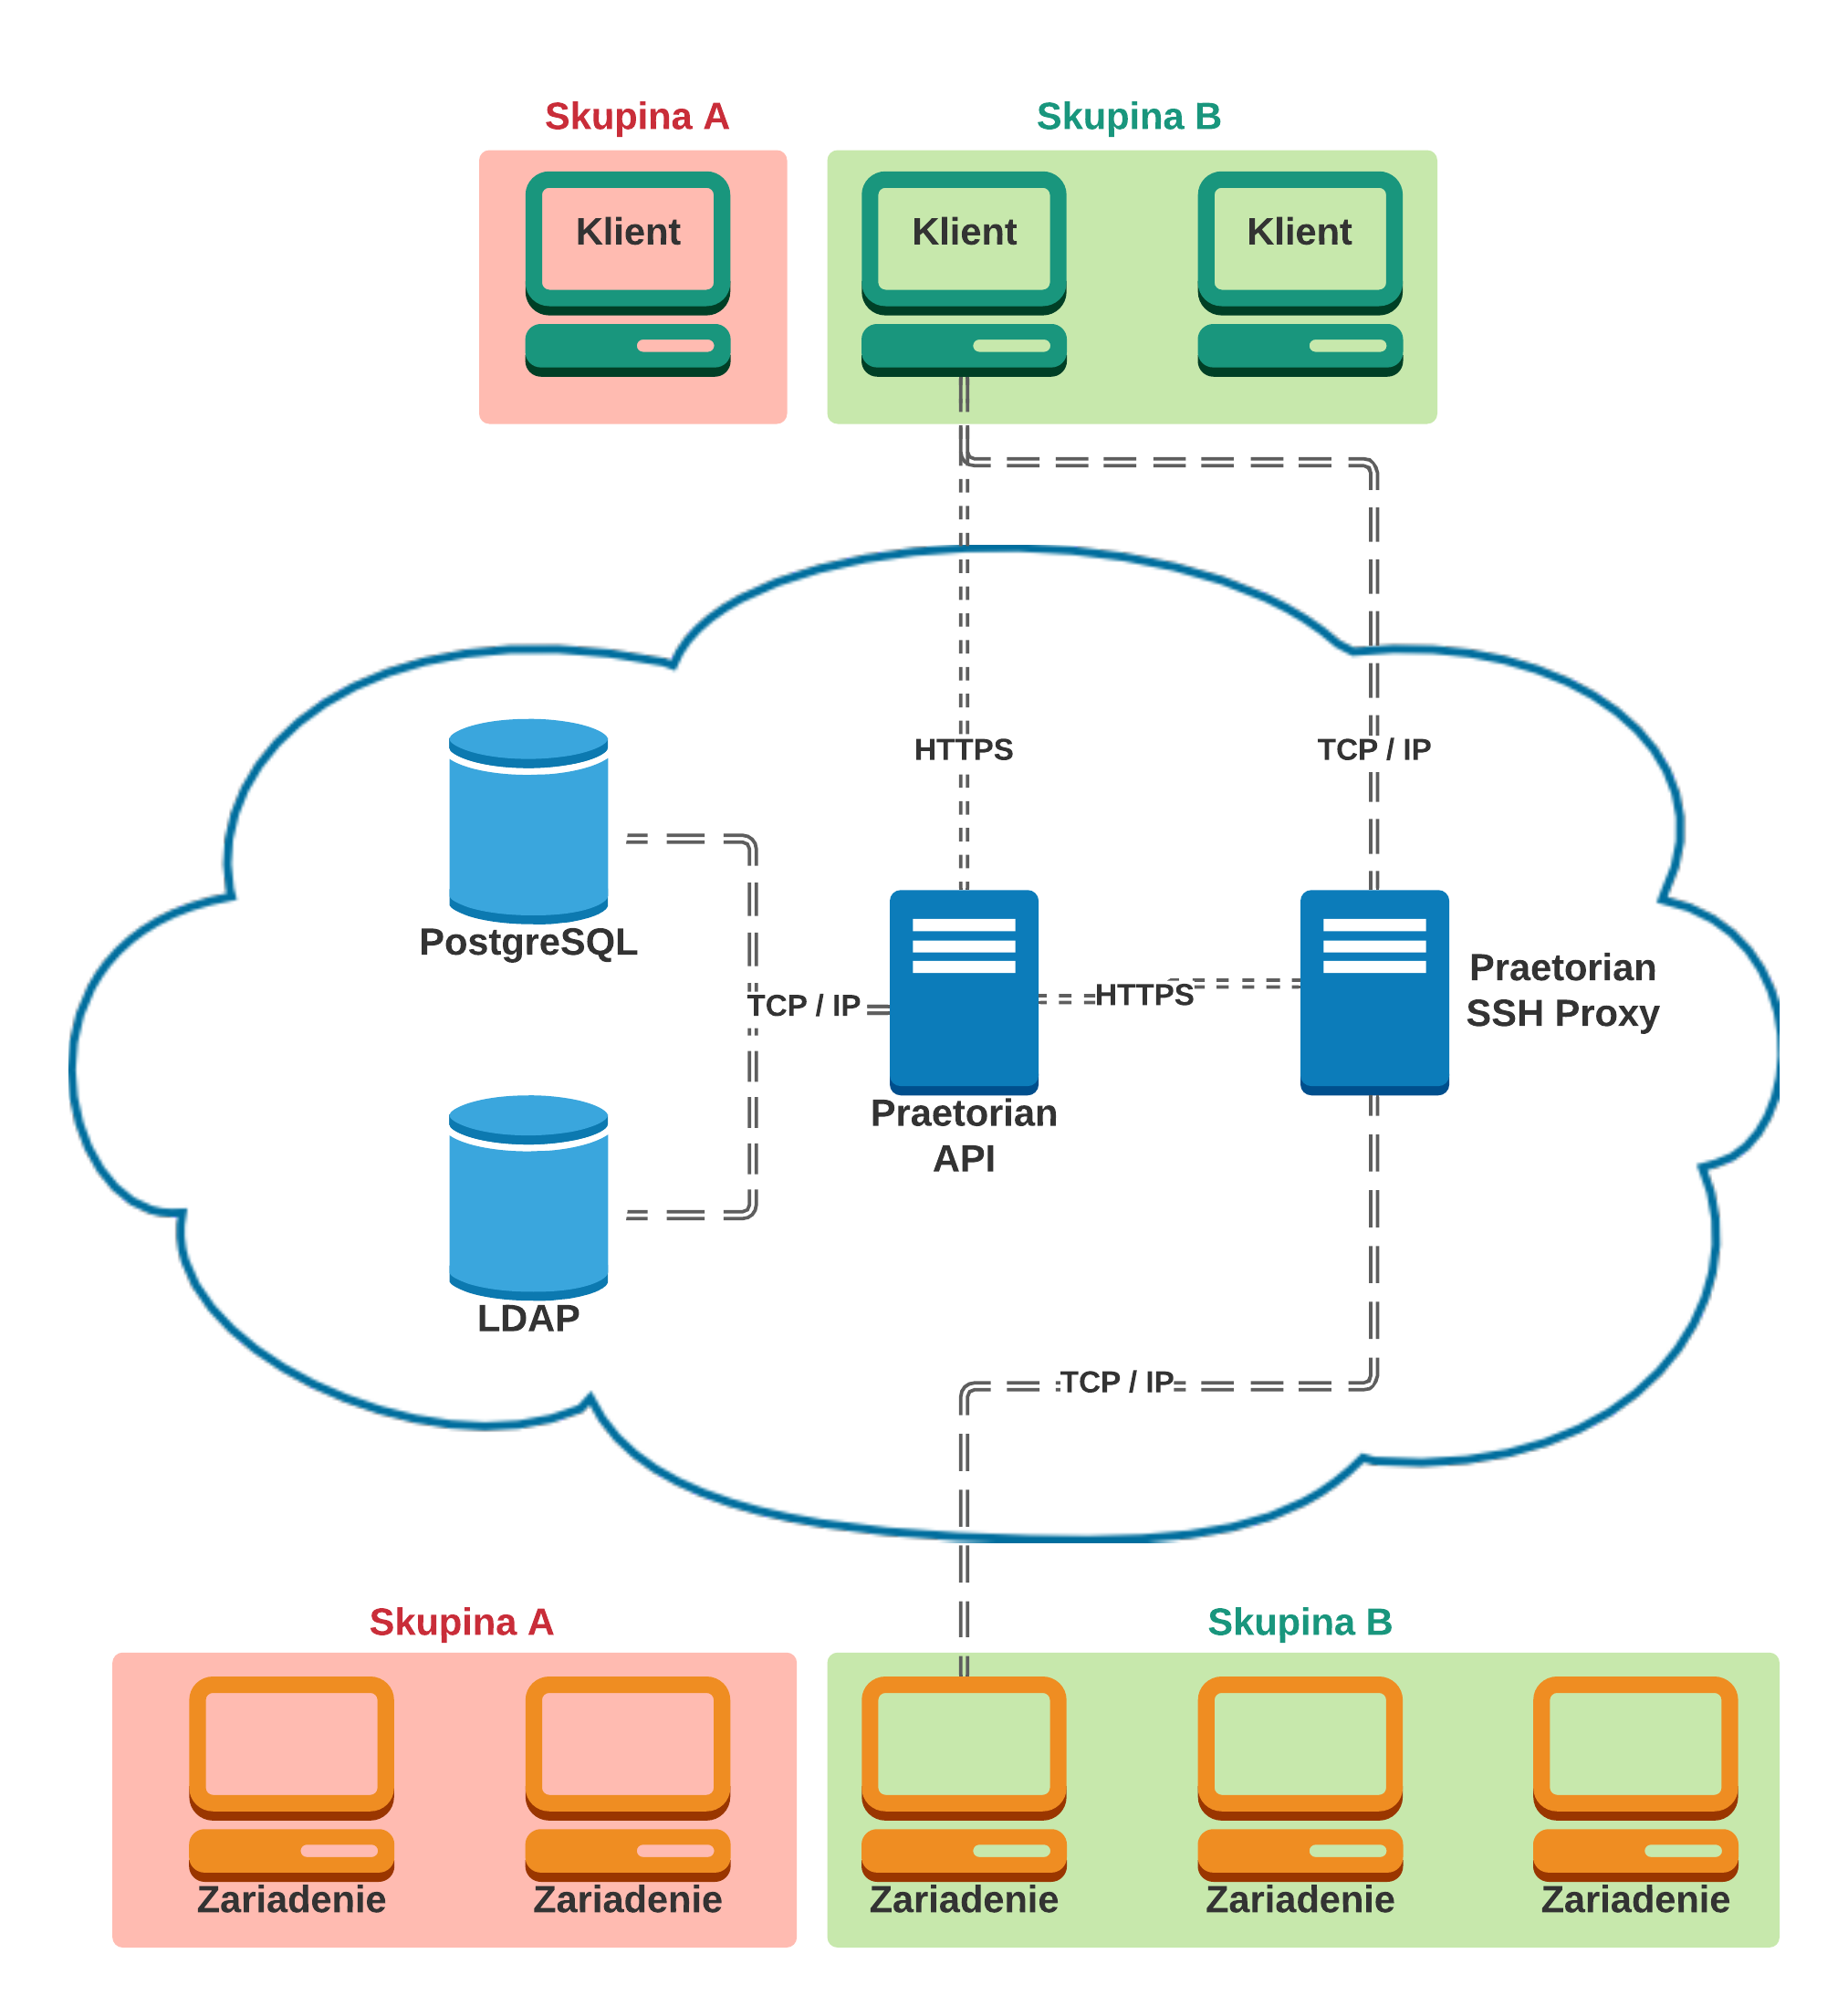
\includegraphics[width=\textwidth,height=12cm,keepaspectratio=true]{assets/demonstracia_riesenia.png}\end{center}
\caption[Náhľad riešenia]{Náhľad riešenia}\label{fig:obr_8}
\end{figure}

Z náhľadu je možné vidieť klientov, ktorí predstavujú bežných používateľov navrhovaného systému.
Môžu sa medzi sebou líšiť svojou rolou v systéme, projektom, ktorý im je pridelený, zoznamom práv a zariadení s ktorými
daný používatelia majú dovolené pracovať, alebo dokonca typom siete, z ktorej sa na daný systém pripájajú.
Všetky tieto aspekty sú systémom sledované a vyhodnocované z pohľadu informačnej bezpečnosti.

Používateľ môže komunikovať s dvoma typmi komponentov.
Prvým je webová aplikácia, ktorá zastrešuje celý systémový manažment, spravuje operácie nad firemnými údajmi a kontroluje
ich správnosť.
Webová aplikácia môže komunikovať s rôznymi typmi dátových úložisk, pričom autentifikácia pokrýva možnosť prihlásenia cez
vnútornú databázu systému, alebo cez protokol ľahkého prístupu k adresáru (Lightweight Directory Access Protocol - LDAP).
To umožňuje jednoduchú správu a migráciu firemných zamestnancov v systéme.
Druhým komponentom je ssh proxy server, ktorého hlavnou úlohou je zabezpečenie komunikácie medzi klientom a vzdialeným
zariadením bez toho, aby obe komunikujúce strany o sebe vedeli.
Komponent funguje, ako tretia strana anonymizujúca a kontrolujúca celý komunikačný proces medzi dvoma bodmi, s možnosťou
auditovateľnosti posielaných správ, či ich filtrovania podľa presne nastavených noriem (ako napríklad whitelist, alebo blacklist).
Taktiež významnou úlohou ssh proxy servera je možnosť bezpečnej komunikácie s webovým api, pričom komunikácia predovšetkým
slúži na kontrolu a validáciu procesu autentifikácie, autorizácie, alebo správu privilegovaného prístupu k potrebným citlivým
údajom za pomoci vlastného špecializovaného api kľúča.

Práve tento nami navrhnutý ssh proxy server umožňuje kľúčovú funkcionalitu, ktorou sa naša práca výrazne odlišuje oproti
existujúcim riešeniam.
Tou je automatizované nasadenie produktu a komunikácia s koncovými zariadeniami bez potreby používateľa akýmkoľvek spôsobom pristúpiť,
alebo interagovať s citlivými a prístupovými údajmi.
Zahájenie tohto druhu operácie si vyžaduje adresu, port ssh proxy servera a osobné prístupové údaje používateľa do systému.
Prístupovými údajmi je možné na strane api servera skontrolovať používateľovu identitu a oprávnenia týkajúce sa miery manipulácie
medzi daným projektom, koncovým zariadením, sieťou, z ktorej sa daná operácia uskutočňuje a zariadením, z ktorého sa akcia vykonáva.
Citlivé údaje sú v databáze systému uložené spôsobom názov-hodnota, pričom k hodnotám má podľa miery dôveryhodnosti prístup buď
iba ssh proxy server, alebo aj samotný používateľ.
Validácia prístupu k týmto údajom je umožnená za pomoci rozdielnych api kľúčov, ktoré sú vyhodnocované api serverom.
Zatiaľ, čo hodnoty citlivých údajov podliehajú validácii, názvy sú používateľovi známe aj pri dôverných (skrytých) informáciach.
Jednotlivé príkazy, ktoré majú obsahovať hodnoty citlivých údajov používateľ nahradí názvom.
Po odoslaní príkazu je možné zo strany ssh proxy servera vykonať požiadavku na api server pod privilegovaným api kľúčom.
Týmto spôsobom si vie názvy dôverných informácií nahradiť hodnotami, a následne príkaz odoslať na anonymizované koncové zariadenie.
Keďže má ssh proxy server prístup k vzdialeným zariadeniam aj prístupovým údajom na rôzne technológie (dátové úložisko, environment premenné, ldap),
bezpečnosť celého riešenia môže byť zvýšená o dodatočnú funkcionalitu automatizovaného dynamického menenia prístupových údajov
podľa nastaveného časového intervalu.

\section{Diagram komponentov}\label{sec:diagram-komponentov}

S prihliadnutím na veľmi vysokú modularitu a rozšíriteľnosť riešenia bol systém a jeho dôležité komponenty dopodrobna rozanalyzovaný.
Médiom znázorňujúcim závislosti medzi softvérovými komponentami, ako napríklad triedy a ich navrhovaný vzťah medzi
nimi sa nazýva diagram komponentov.
Keďže sa jedná o veľmi komplexné riešenie, prihliadali sme z dôvodu prehľadnosti na abstrahovanie problému v čo najvyššej miere.
Výsledný diagram komponentov~\ref{fig:obr_9}~zobrazený nižšie, znázorňuje vzťahy tých komponentov, ktoré sú nevyhnutné pre
získanie vzdialeného prístupu ku koncovému zariadeniu.

\begin{figure}[H]
\begin{center}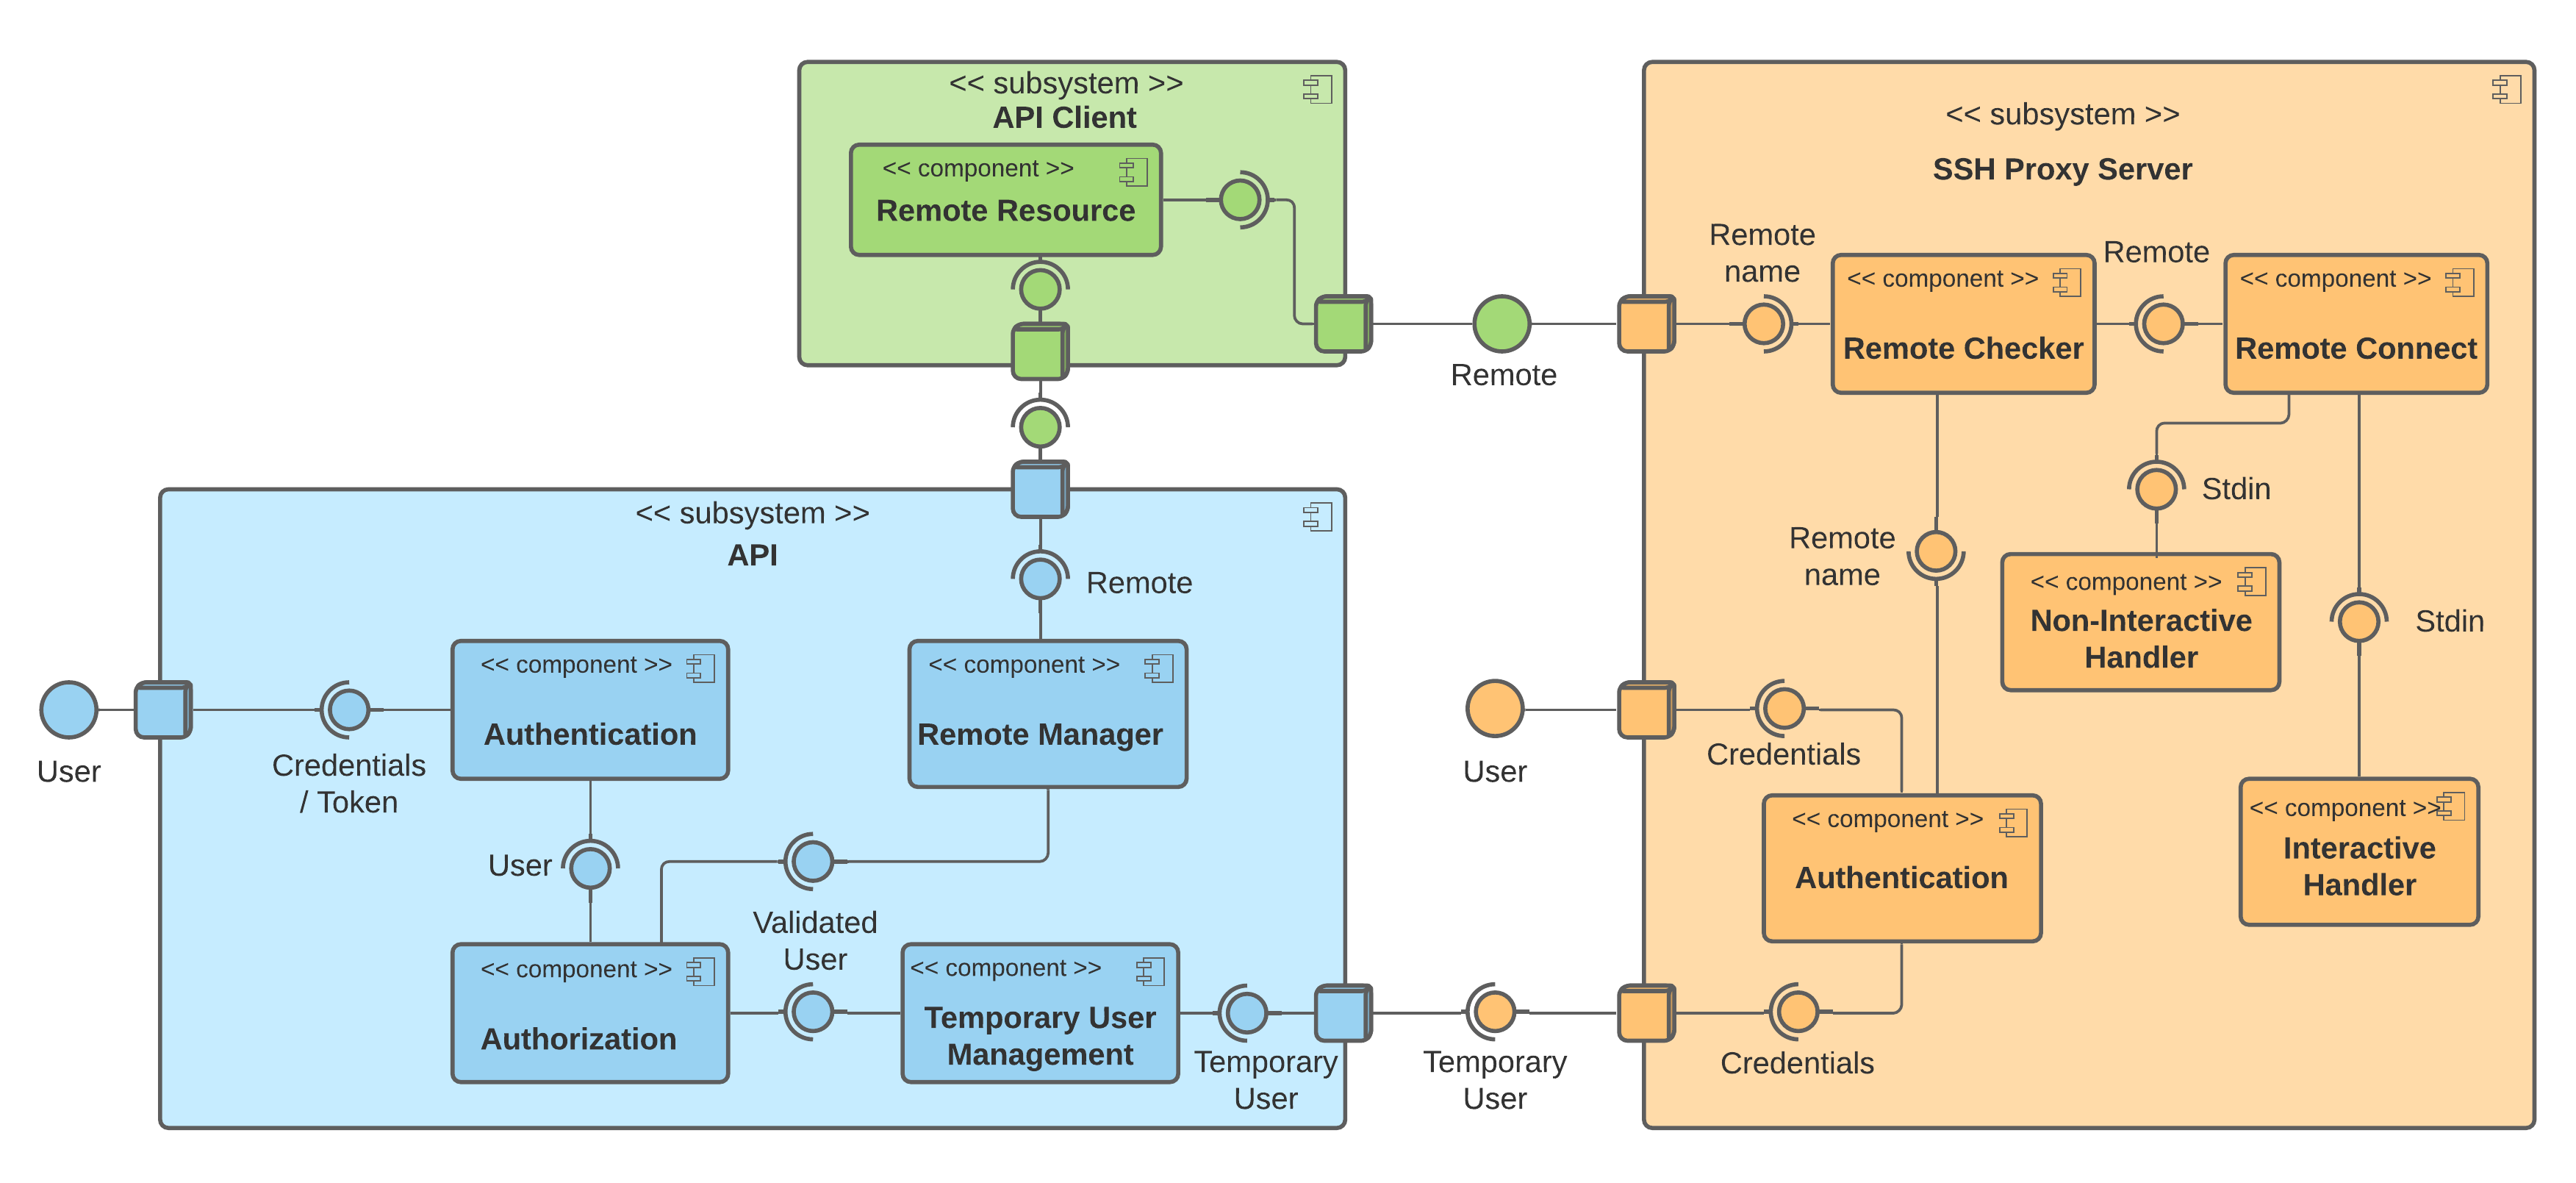
\includegraphics[width=\textwidth,height=8cm,keepaspectratio=true]{assets/diagram_komponentov.png}\end{center}
\caption[Diagram komponentov]{Diagram komponentov}\label{fig:obr_9}
\end{figure}

Ako je v diagrame znázornené, celý navrhovaný systém sa skladá z troch hlavných komponentov: webové api, api klient a ssh proxy server.
Komunikácia medzi webovým api a ssh proxy serverom prebieha cez api klienta, ktorý zvyšuje modularitu, bezpečnosť, udržiavateľnosť a
auditovateľnosť celého riešenia.
V systéme figurujú dva hlavné typy používateľov, a to štandardný permanentný používateľ, ktorý sa môže prihlásiť do webovej
aplikácie a súčasne, ak je mu to oprávnené, môže komunikovať so vzdialeným zariadením cez ssh proxy server v interaktívnej
relácii ssh (interactive ssh session).
Druhým typom používateľa je dočasný, ktorého životnosť po vytvorení vo webovej aplikácii trvá iba obmedzený čas, alebo jeho
životnosť je ukončená súčasne s dokončením úlohy, pre ktorú bol vytvorený.
Dočasného používateľa je možné vytvoriť iba permanentným používateľom s prislúchajúcim oprávnením, pričom dočasný
používateľ je vytváraný s jediným cieľom, a tým je pripojenie sa na konkrétne vzdialené zariadenie.
Preto po tvorcovi „zdedí“ zvolený projekt a prístup ku konkrétnemu vzdialenému zariadeniu.
Tvorcovi následne príde notifikácia vo forme emailu o prístupových údajoch dočasného používateľa, pod ktorým je môže vykonať príkazy
v neinteraktívnej relácii ssh (non-interactive ssh session) cez ssh proxy server na koncové zariadenie.

\section{Sekvenčné diagramy}\label{sec:sekvencne-diagramy}

Keďže sa naše riešenie vo veľkej miere zaoberá vzájomnou komunikáciou medzi jednotlivými komponentami celého systému, je
veľmi dôležité pri návrhu zachytiť procesy, ktoré sa vykonávajú sekvenčne pri komunikácii.
Väčšina týchto procesov figuruje vo forme správ, ktoré si jednotlivé komponenty vymieňajú, a preto bolo pri návrhu daných
častí systému použitie sekvenčných diagramov optimálnou voľbou.

\subsection{Autentifikácia}\label{subsec:sek-autentifikacia}

Prvý sekvenčný diagram~\ref{fig:obr_10}~znázorňuje autentifikáciu prístupu používateľa k navrhovanému ssh proxy serveru.
Z pohľadu servera sa jedná o autentifikáciu klienta, ktorý môže byť permanentného, aj dočasného typu a taktiež musí patriť
do daného bezpečnostného systému.
Pre pripojenie k ssh proxy serveru je taktiež potrebné zistiť k akému koncovému zariadeniu sa používateľ chce pripojiť a
voči tomuto zvolenému zariadeniu skontrolovať autorizáciu pripájaného klienta.

\begin{figure}[H]
\begin{center}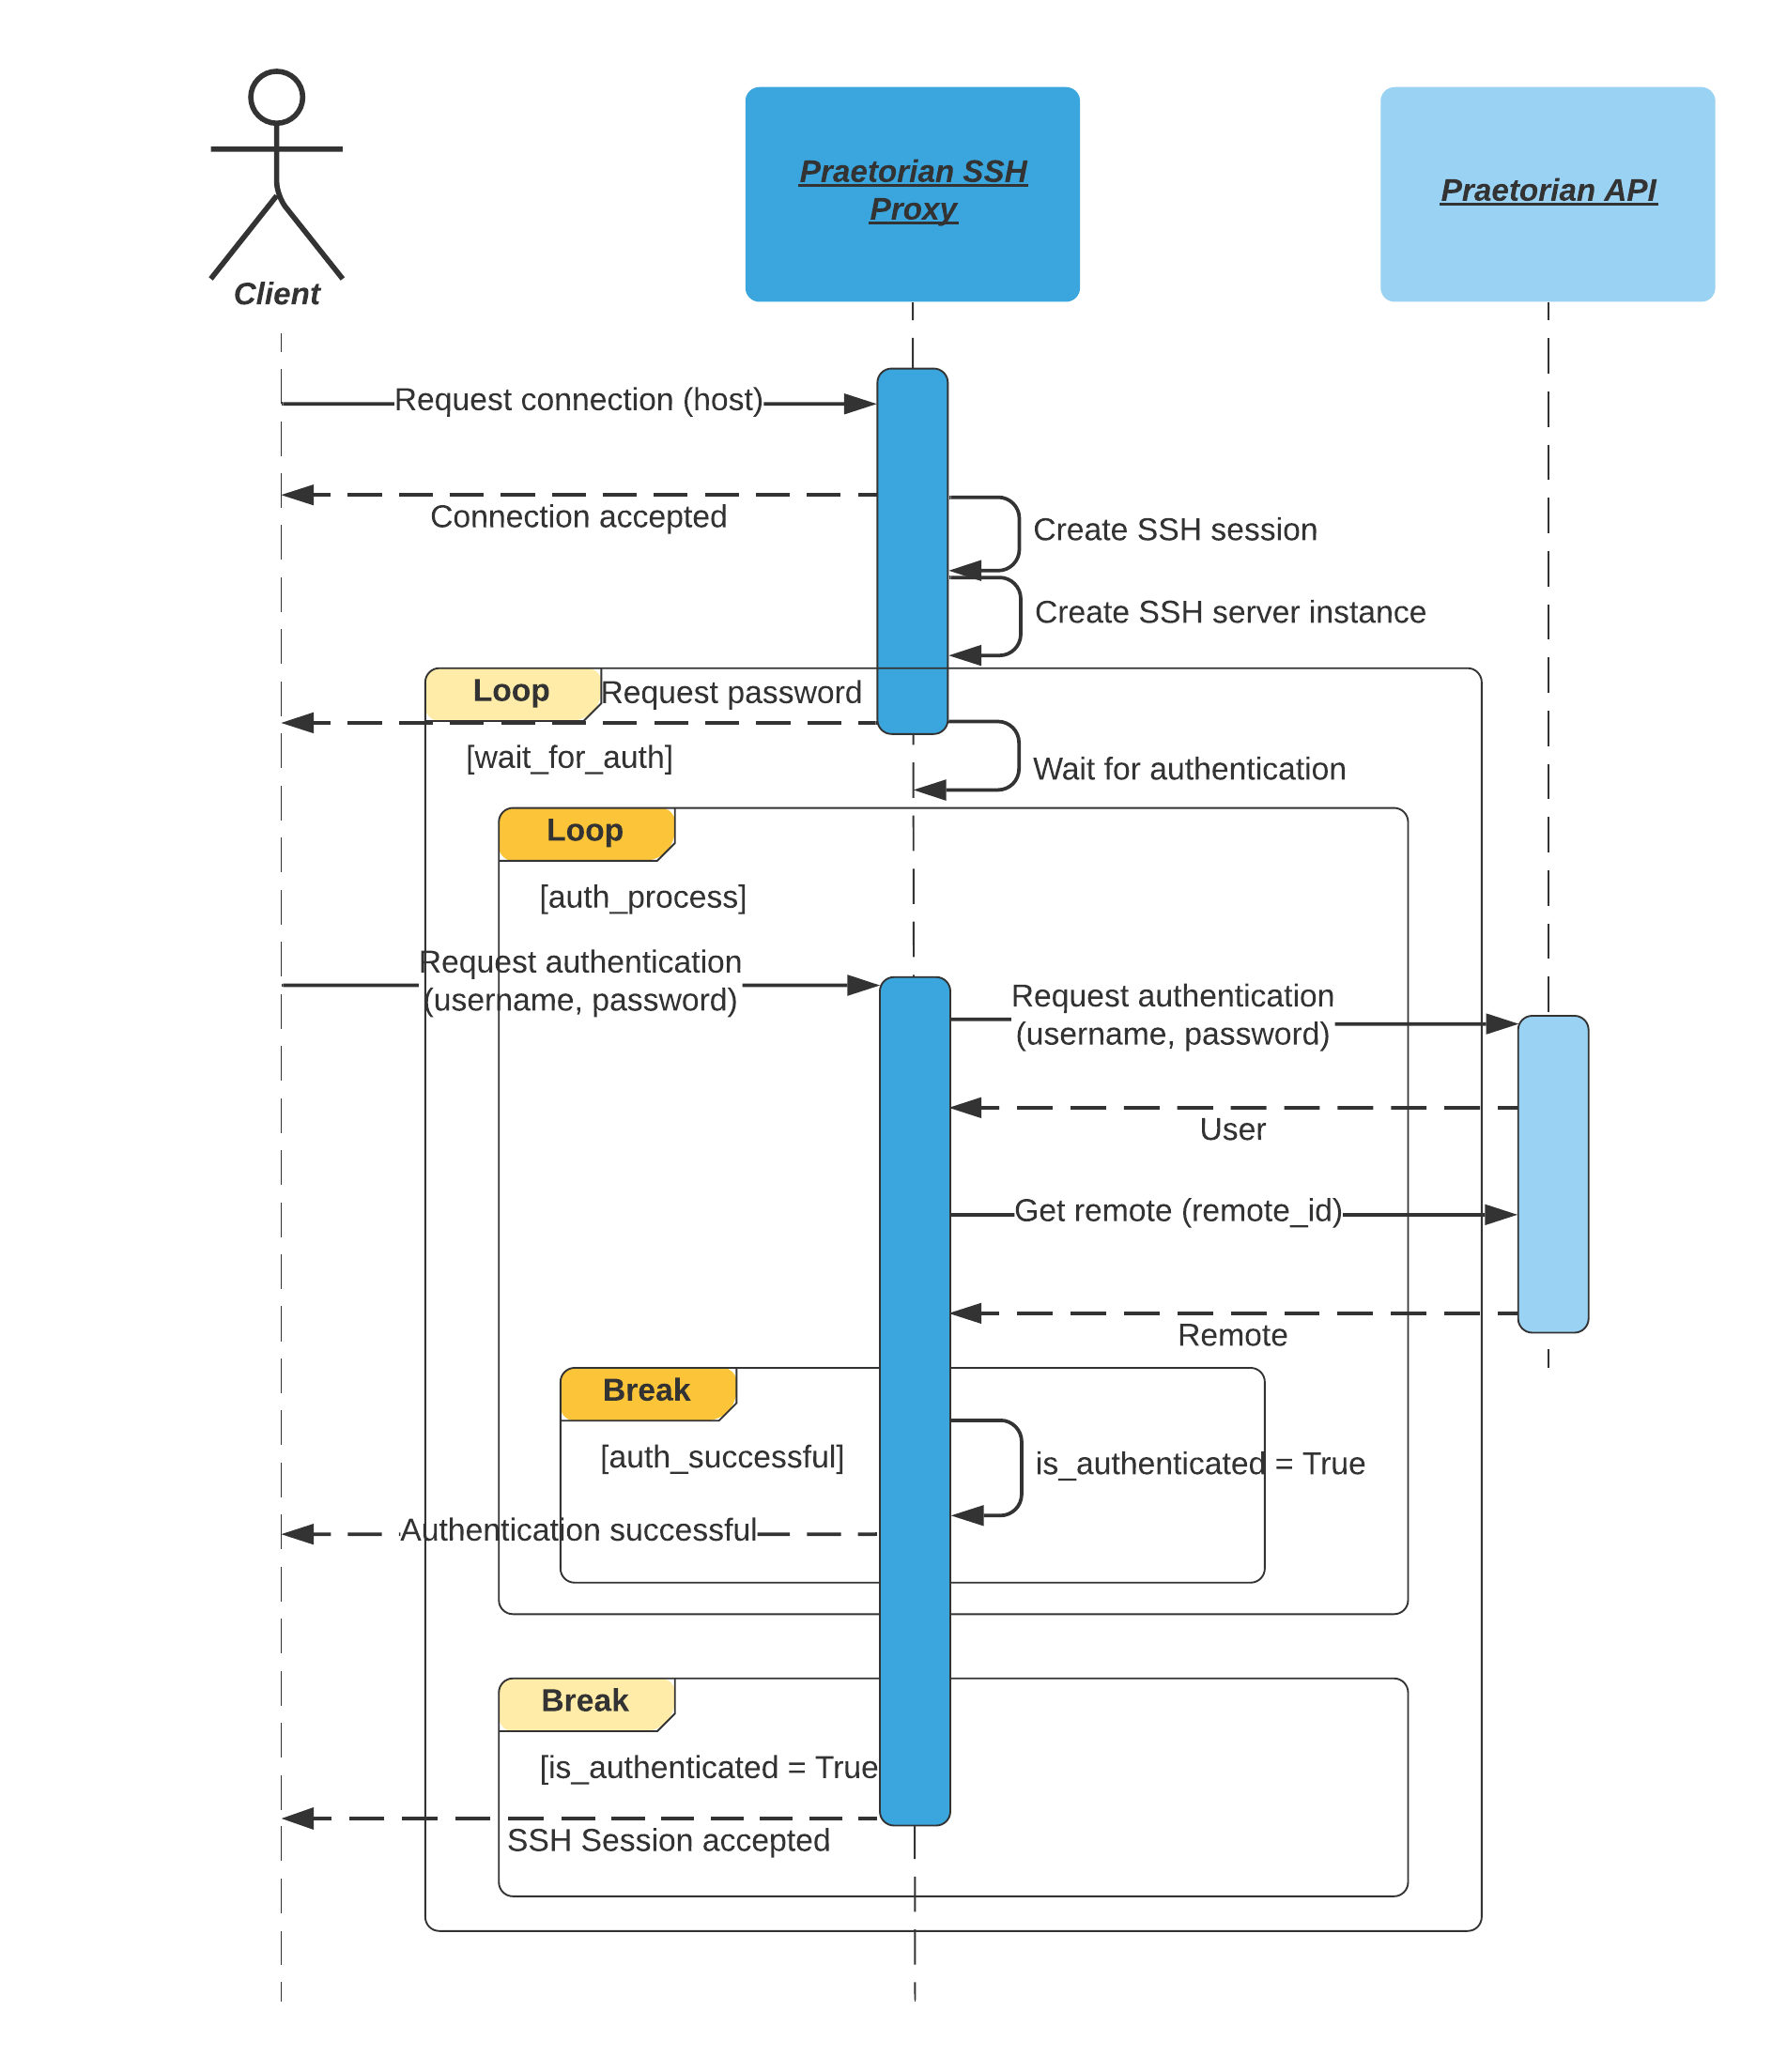
\includegraphics[width=\textwidth,height=15cm,keepaspectratio=true]{assets/sequence_diagram_auth.png}\end{center}
\caption[Autentifikácia]{Autentifikácia}\label{fig:obr_10}
\end{figure}

Ak sa chce klient pripojiť k ssh proxy serveru s úmyslom pripojenia sa na vzdialené zariadenie, musí si k serveru vyžiadať
prístup.
Po vyžiadaní prístupu server príjme daného klienta, umožnením komunikácie cez soket s cieľom otvorenia spojenia ssh.
Preto server vytvorí po pripojení klienta na daný soket novú ssh reláciu (ssh session) a následne vytvorí rozhranie ssh servera,
ktorého úlohou je spracovať vstup od klienta cez dané spojenie.
Proces vytvorenia rozhrania servera zároveň pošle klientovi požiadavku pre overenie pomocou hesla, pričom server čaká, dokiaľ
sa používateľ úspešne autentifikuje, alebo ukončí spojenie.
Po úspešnom zaslaní hesla, začína autentifikačný proces na strane servera, ktorý si overí správnosť pripájaného klienta vytvorením
novej inštancie api klienta s daným menom a heslom používateľa.
Ak sa api klient inštancia úspešne prihlási do webového api, ssh proxy server si cez api klienta vypýta dodatočné informácie o
používateľovi a koncové zariadenie.
Ak sú získané údaje z webového api validné, potom je autentifikácia úspešne ukončená a ssh relácia zo strany servera úspešne akceptovaná.

\subsection{Interaktívne prostredie}\label{subsec:interkativne-prostredie}

Druhý sekvenčný diagram~\ref{fig:obr_11}~zobrazuje proces vytvorenia a spracovania interaktívneho rozhrania ssh.
Tento typ pripojenia je umožnený iba permanentným používateľom systému a iba ku koncovým zariadeniam, ku ktorým majú daný
používatelia prístup.
Interaktívne prostredie ssh umožňuje simulovanie terminálu vzdialeného zariadenia, pričom pripojený používateľ môže v reálnom
čase posielať na dané zariadenie vstup vo forme príkazov, ktorých výstup im je následne zobrazovaný na výstupe.

\begin{figure}[H]
\begin{center}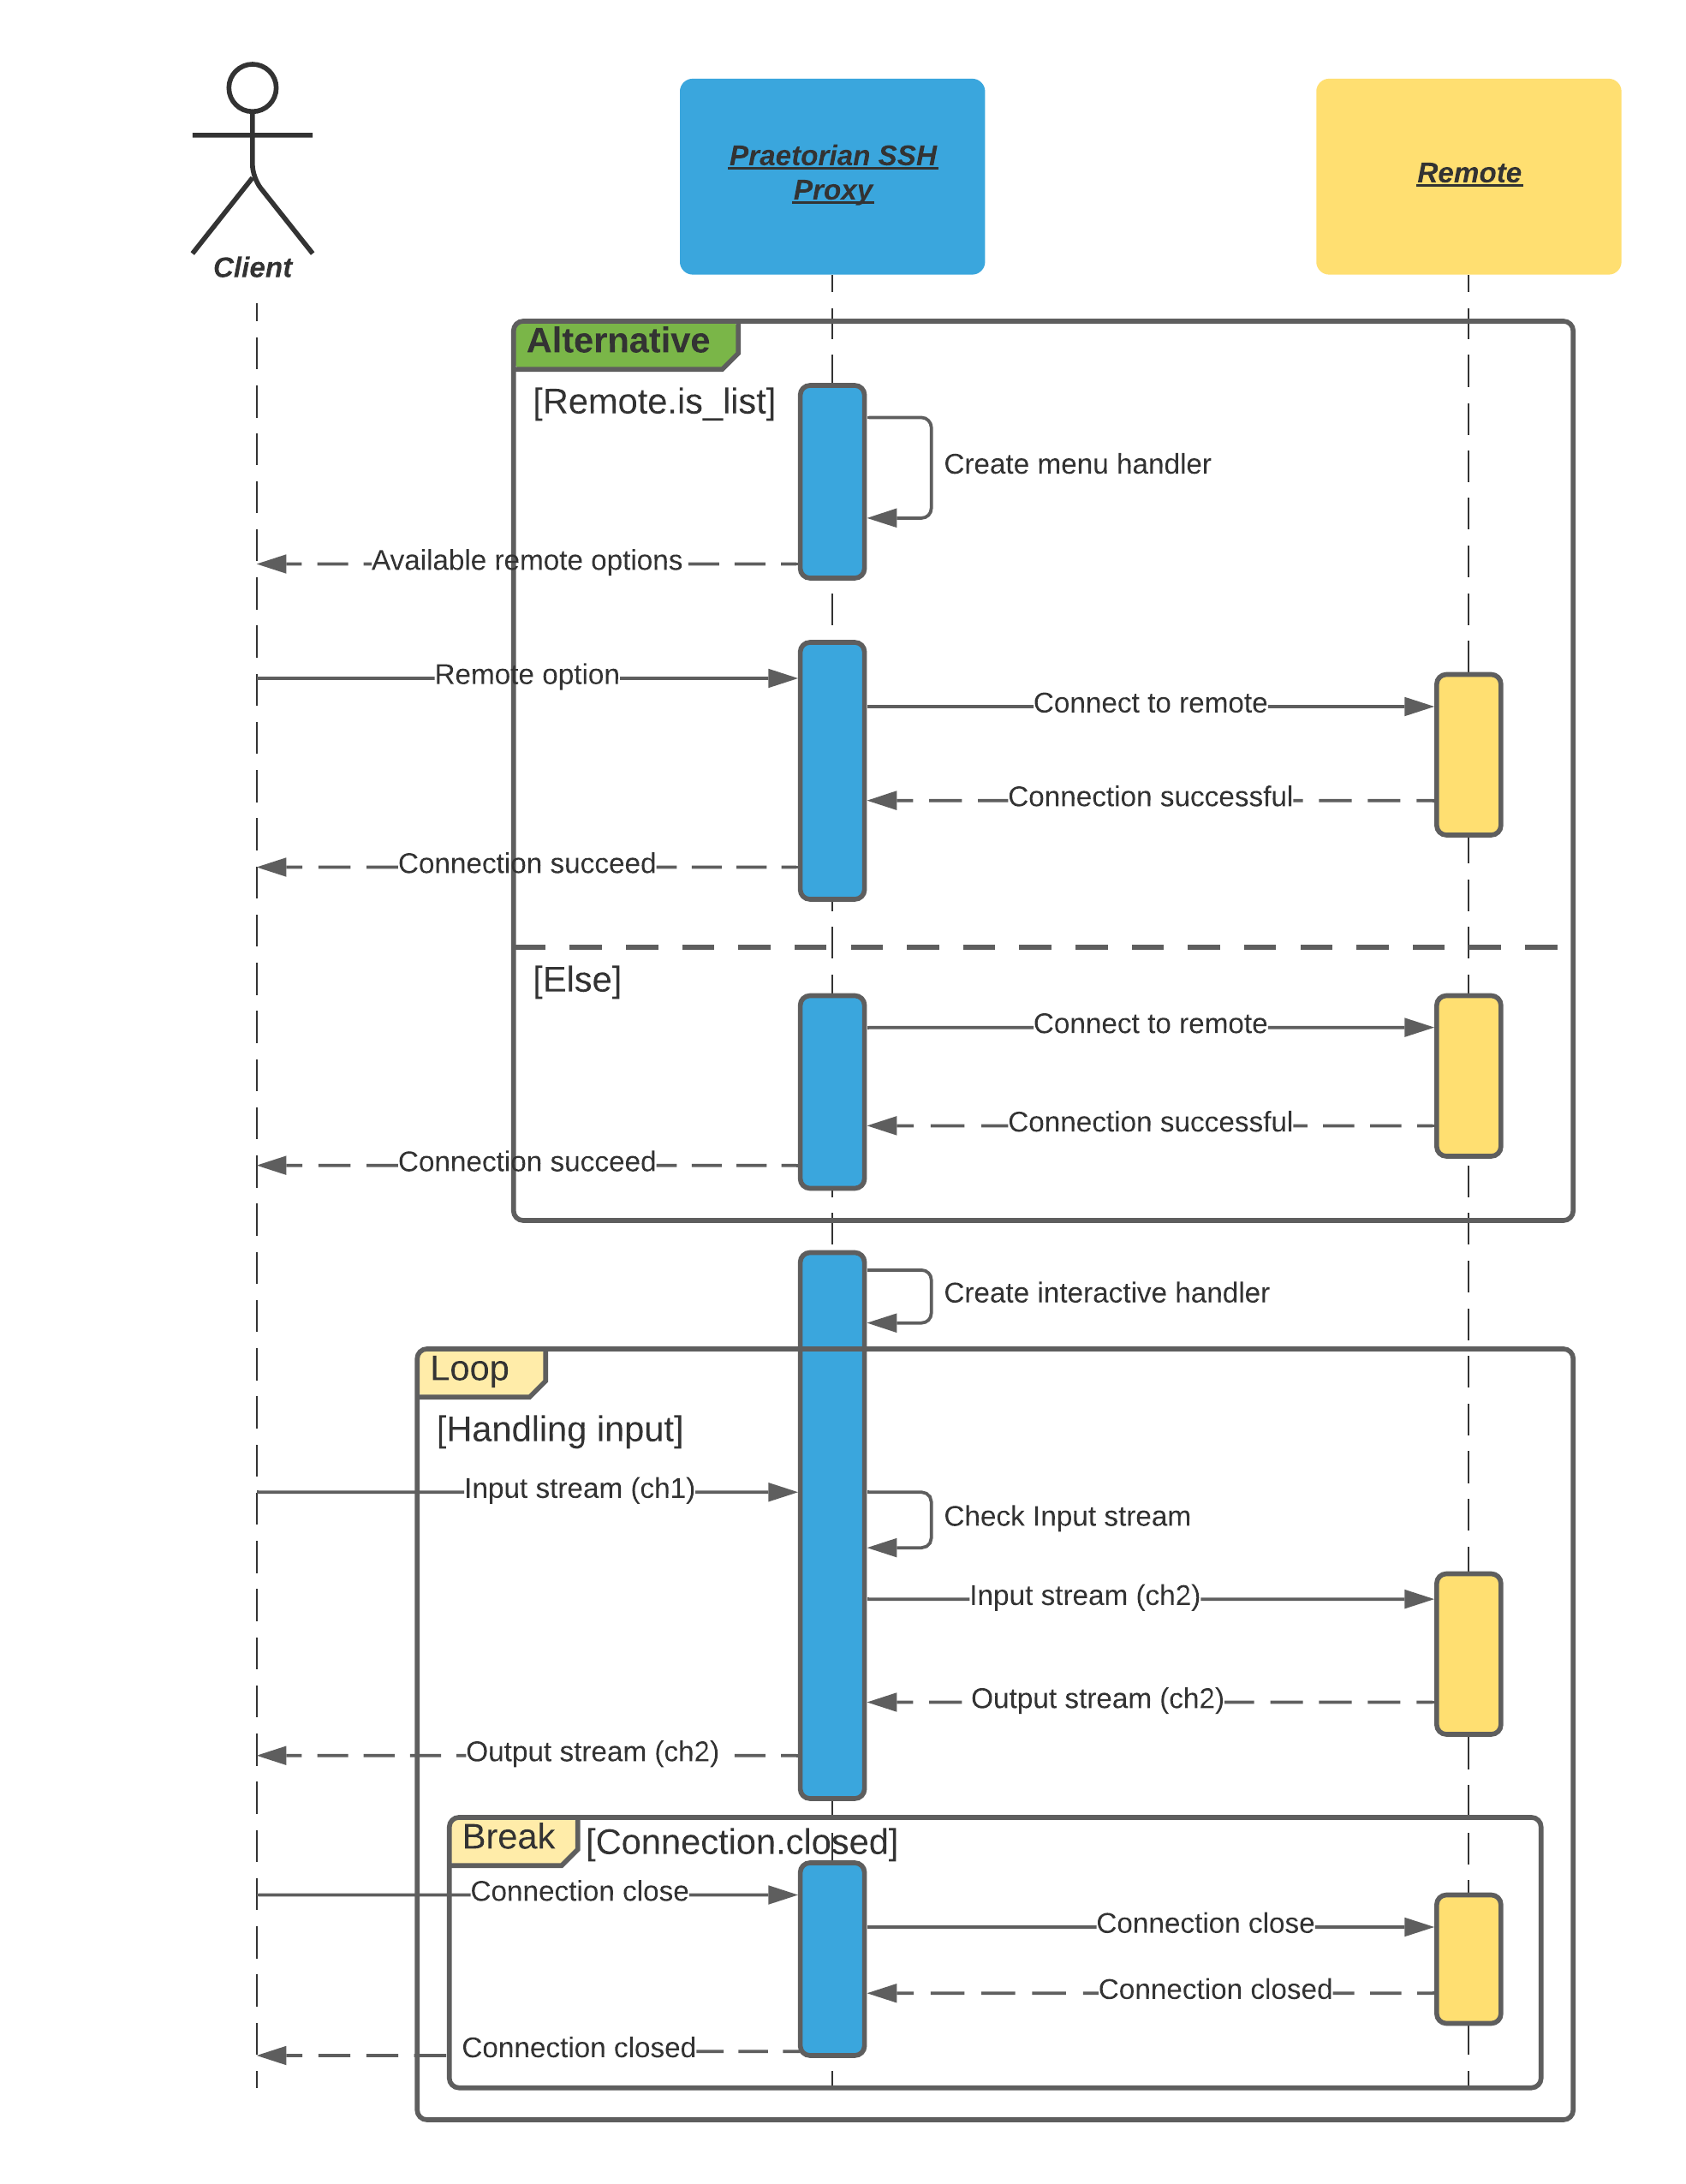
\includegraphics[width=\textwidth,height=15cm,keepaspectratio=true]{assets/sequence_diagram_interactive.png}\end{center}
\caption[Interaktívne prostredie]{Interaktívne prostredie}\label{fig:obr_11}
\end{figure}

Ak je úspešne autentifikovaný klient permanentným používateľom, má po pripojení k ssh proxy serveru dve možnosti.
Prvou je špecifikovanie vzdialeného zariadenia, ku ktorému sa chce klient pripojiť, alebo nešpecifikovať žiadne.
V prípade druhej z možností sa na strane ssh proxi servera vytvorí inštancia triedy „MenuHandler“, ktorá si z webového api
vyžiada zoznam dostupných koncových zariadení ku ktorým má daný používateľ právo.
Vytvorená inštancia následne vytvorí menu, z ktorého si používateľ môže vybrať práve jedno dané zariadenie.
Následne po vybraní zariadenia, proxy server požiada ssh server zariadenia o pripojenie s cieľom vzájomnej komunikácie.
Po úspešnom nadviazaní spojenia, proxy server vytvorí inštanciu triedy „InteractiveHandler“, ktorá zabezpečuje simuláciu
terminálu vzdialeného zariadenia.
Úlohou danej inštancie proxy servera je preposielanie vstupu z klienta na koncové zariadenie a spätné preposielanie výstupu
klientovi dovtedy, dokiaľ klient nepožiada o ukončenie spojenia.
Po vyžiadaní ukončenia spojenia zo strany klienta sa proxy server pokúsi uzavrieť spojenie so vzdialeným zariadením a nakoniec
uzavrie spojenie so samotným klientom.

\subsection{Neinteraktívne prostredie}\label{subsec:neinterkativne-prostredie}

Narozdiel od interaktívneho rozhrania, neinteraktívne rozhranie nesimuluje posielanie príkazov v reálnom čase, no slúži na
sekvenčné zaslanie príkazov pomocou skriptu, alebo súboru, pričom pri úspešnom dokončení sa spojenie ukončí a uzavrie.
K takémuto typu prostredia majú prístup iba dočasní používatelia, ktorý budú po vykonaní danej úlohy a po úspešnom ukončení spojenia
vymazaný.
Nasledujúci sekvenčný diagram~\ref{fig:obr_12}~graficky zobrazuje postup použitia daného prostredia, no taktiež pre úplnosť
celého postupu pri pripojení klienta na ssh proxy server obsahuje referencie na predchádzajúce dva sekvenčné diagramy.

\begin{figure}[H]
\begin{center}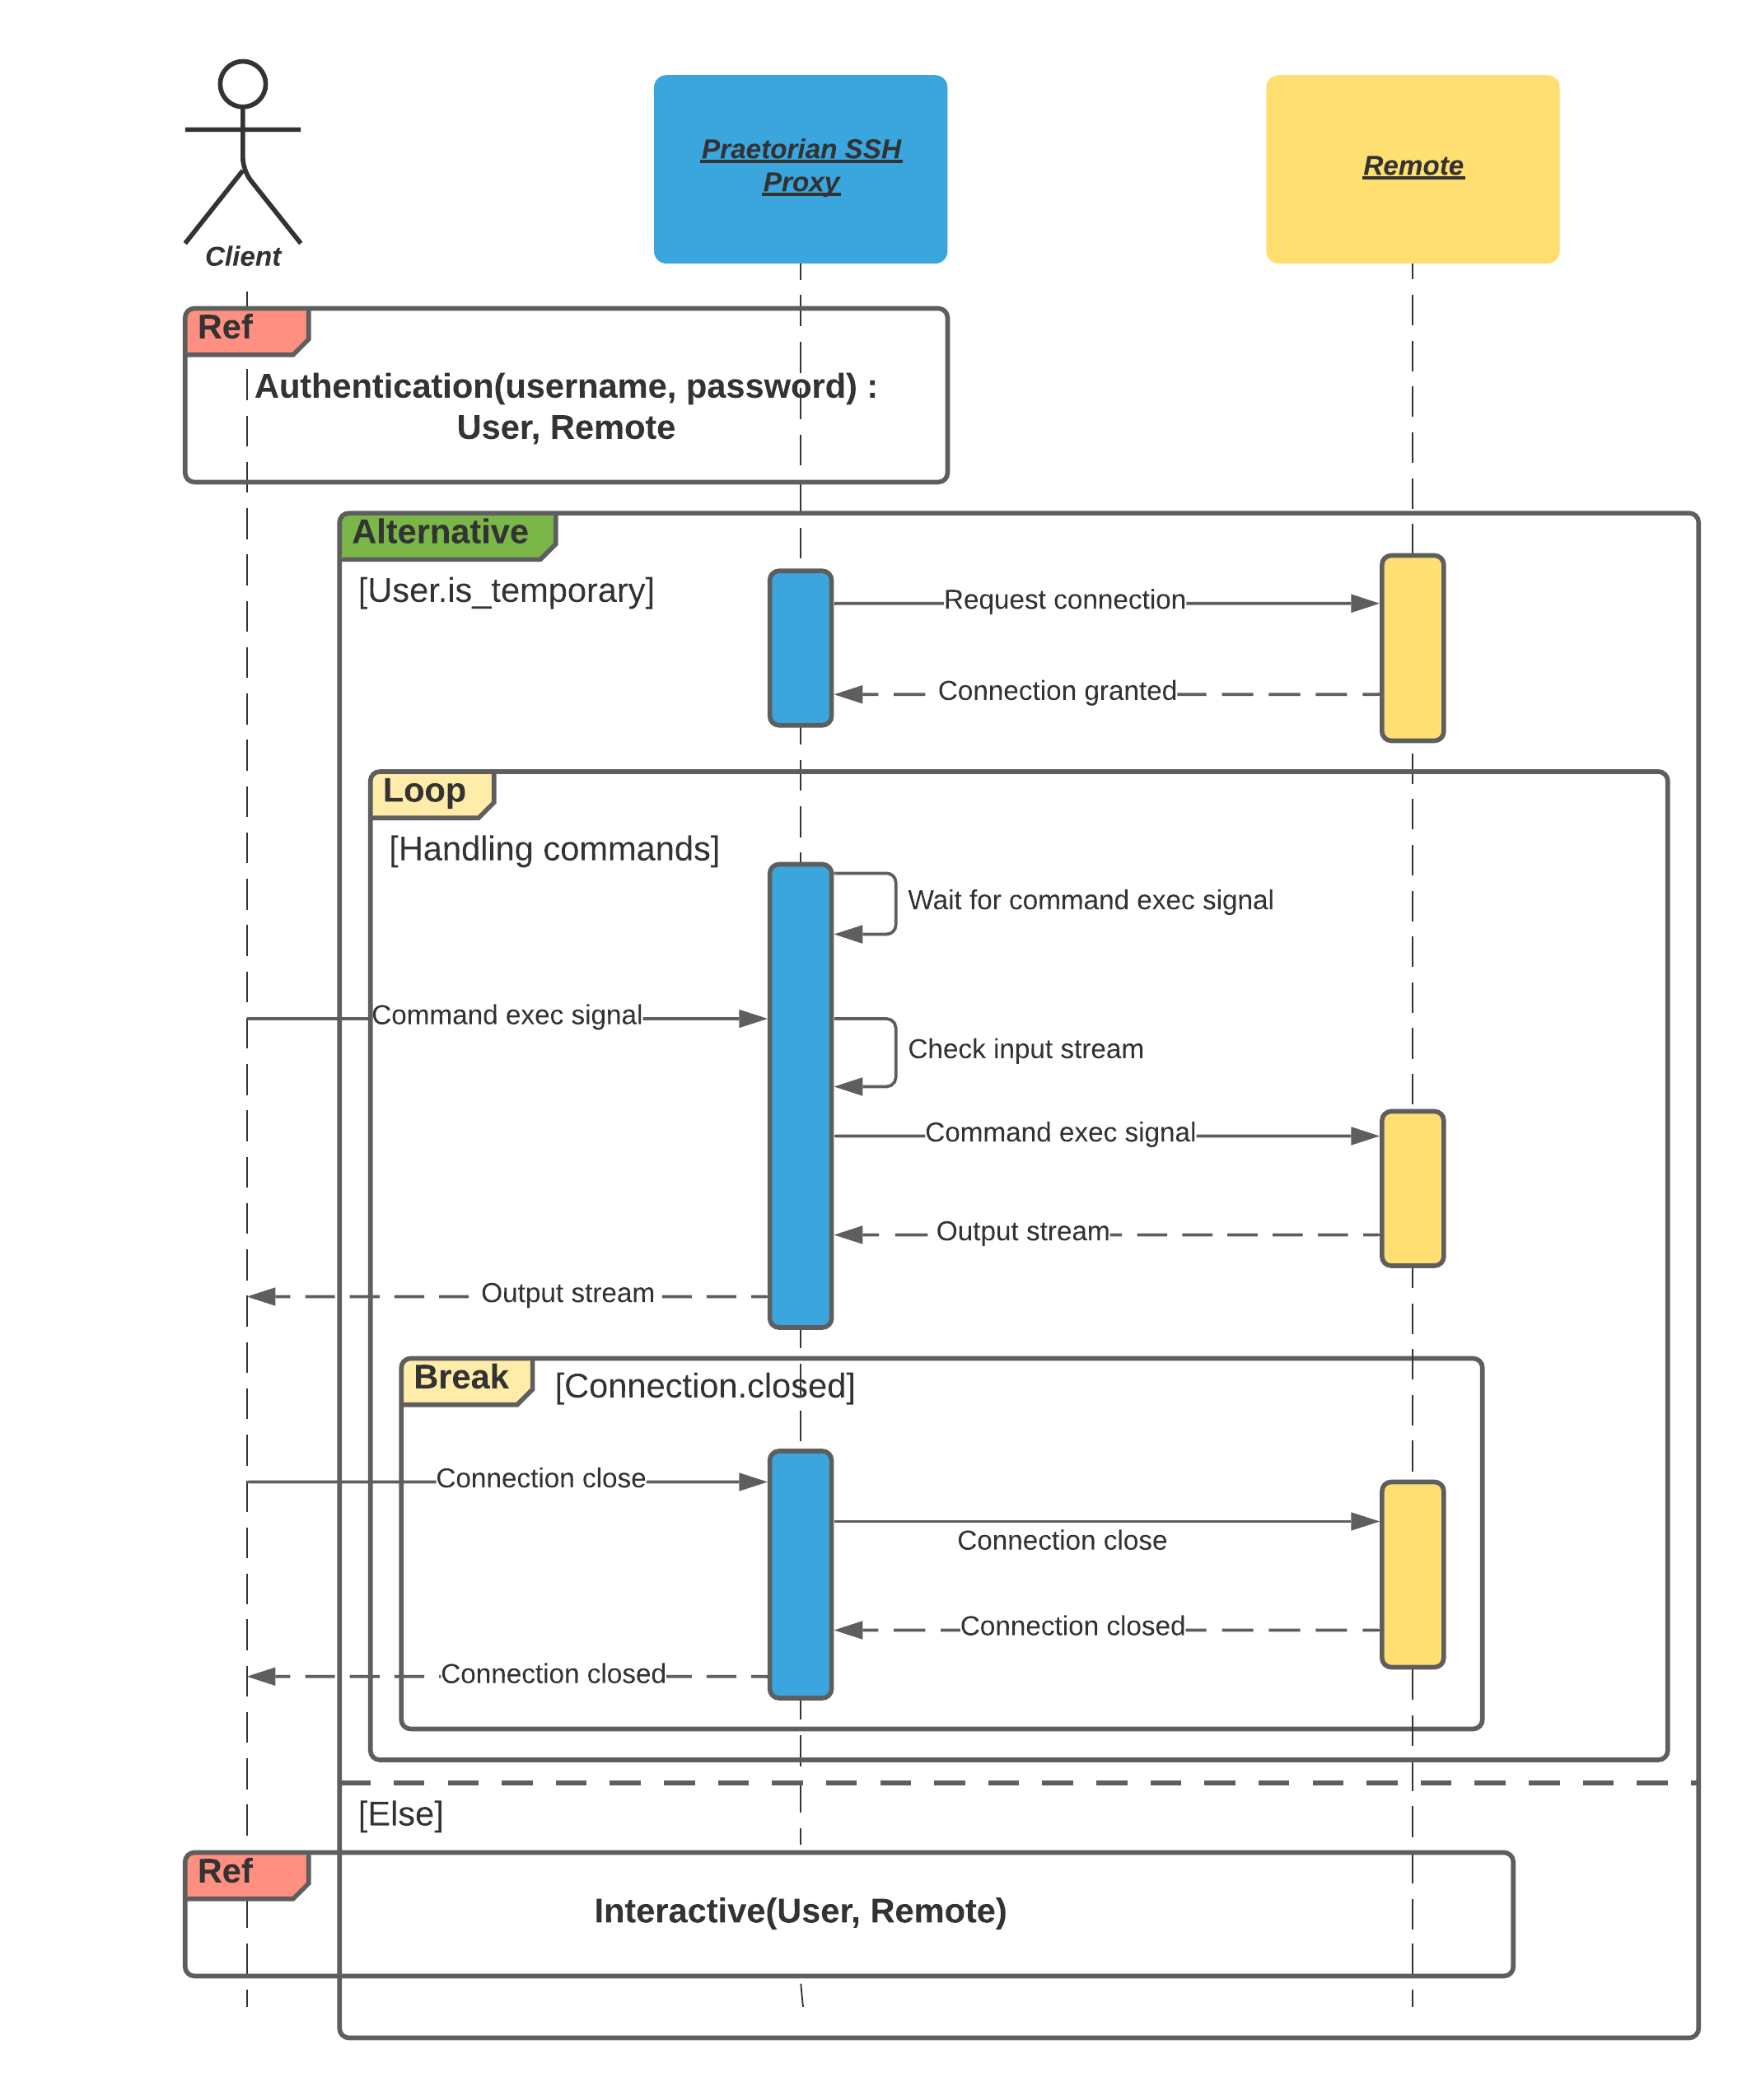
\includegraphics[width=\textwidth,height=15cm,keepaspectratio=true]{assets/sequence_diagram_non_interactive.png}\end{center}
\caption[Neinteraktívne prostredie]{Neinteraktívne prostredie}\label{fig:obr_12}
\end{figure}

Po úspešnom overení dočasného používateľa, je koncové zariadenie, na ktoré sa chce pripojiť známe, keďže dočasného používateľa
nie je možné vytvoriť na strane webovej aplikácie bez špecifikovania práve jednoho koncového zariadenia.
Tým pádom hneď po úspešnom overení totožnosti používateľa, si ssh proxy server vyžiada pripojenie na vzdialené zariadenie.
Po úspešnom pripojení k zariadeniu proxy server začne čakať na prípadné vstupy od klienta vo forme shell príkazu.
Akonáhle dostane správu, príkaz skontroluje, či neporušuje pravidlá bezpečnosti a následne ho prepošle ako príkaz do ssh
servera vzdialeného zariadenia.
Následne proxy server počká na odpoveď, ktorú po prijatí prepošle ako odpoveď klientovi.
Proxy server bude čakať a preposielať príkazy dovtedy, dokiaľ klient nepožiada o ukončenie spojenia.
Po prijatí ukončenia spojenia od klienta, proxy server pošle požiadavku o ukončenie spojenia ssh serveru koncového zariadenia
a po úspešnom uzavrení spojenia proxy server uzavrie spojenie aj s klientom.
Dané neinteraktívne rozhranie je možné použiť na veľa spôsobov, ako napríklad spracovanie skriptu, alebo súboru s príkazmi,
či pracovať so systémami, ktoré potrebujú pripojenie na ssh.

\chapter{Vyhodnotenie navrhovaného riešenia}\label{ch:vyhodnotenie-navrhovaneho-riesenia}

Primárnym výsledkom nášho navrhovaného riešenia bolo zabezpečenie prístupu na vzdialené zariadenie.
Samotný prístup na koncové zariadenia musí spĺňať bezpečnostné požiadavky vo všetkých fázach implementovaného prípadu
použitia.
Ďalším dôležitým cieľom bolo zaistenie komunikácie medzi jednotlivými časťami systému a modulárne navrhnúť všetky potrebné
súčasti tak, aby ich bolo možné s pribúdajúcimi kritériami bezpečnosti, alebo použitia jednoducho doimplementovať.

Pri nasadení nášho riešenia, v systéme figuruje iba používateľ typu „superuser“, ktorý má všetky systémové práva.
Tento používateľ vie vytvoriť potrebné záznamy, ako napríklad: projekty, koncové zariadenia, role, používateľov, a ďalšie,
ktoré sú nevyhnutné pre správne fungovanie systému.

Vytvorenie používateľa s rolou „devops“ je po prihlásení superuserom nasledovné:
\newpage
\textbf{\large Požiadavka [POST]:}

\begin{lstlisting}[language=json,firstnumber=1]
{
  "email": "devops@praetorian.sk",
  "password": "devops",
  "name": "devops",
  "surname": "devops",
  "role": "devops",
  "is_vpn": false,
  "additional_data": {},
  "language_id": "ee3f8e7a-c9d8-4d96-8dd0-816775b25b7d"
}
\end{lstlisting}

\textbf{\large Odpoveď:}

\begin{lstlisting}[language=json,firstnumber=1]
{
  "response": {
    "id": "dbab895b-5568-45bf-95a3-55d96118836c",
    "username": "devops@praetorian.sk",
    "name": "devops",
    "surname": "devops",
    "email": "devops@praetorian.sk",
    "phone": null,
    "role": "devops",
    "is_temporary": false,
    "additional_data": {}
  }
}
\end{lstlisting}

Po úspešnom vytvorení používateľa a po registrovaní jeho zariadenia v systéme, je mu možné priradiť superuserom jeden z
existujúcich projektov v systéme a následne sa za neho prihlásiť:

\textbf{\large Požiadavka [POST]:}

\begin{lstlisting}[language=json,firstnumber=1]
{
  "username": "devops@praetorian.sk",
  "password": "devops"
}
\end{lstlisting}

\textbf{\large Odpoveď:}

\begin{lstlisting}[language=json,firstnumber=1]
{
  "response": {
    "token": "22fcf8a5-7c90-4e3a-a665-7cf842b46283",
    "active_2fa": false
  }
}
\end{lstlisting}

Ako je z odpovede webového api rozhrania vidieť, používateľ nie je overený dvojfaktorovou autentifikáciou.
Táto hodnota sa v odpovedi nachádza z dôvodu informovania, či je potrebné vyžiadanie tohto dodatočného typu autentifikácie.

Pre vyžiadanie dvojfaktorovej autentifikácie je potrebné si danú službu aktivovať nasledovným spôsobom:

\textbf{\large Požiadavka [GET]:}

\inlinecode{\{\{ api\_url \}\}/v1/users/\{\{ user\_id \}\}/2fa/}

\newpage
\textbf{\large Odpoveď:}

\begin{lstlisting}[language=json,firstnumber=1]
{
  "response": {
    "qr_code": "otpauth://totp/Praetorian%20API:devops%40praetorian.sk?secret=J4UZONZ36IQGLZAM&issuer=Praetorian%20API"
  }
}
\end{lstlisting}

Reťazec v odpovedi slúži na vytvorenie qr kódu, ktorý bude zobrazený v grafickom užívateľskom rozhraní, pričom používateľ
je taktiež o aktivácii dvojfaktorovej autentifikácie informovaný pomocou zaslaného systémového emailu, ktorého obsah
je na obrázku~\ref{fig:obr_13}.

\begin{figure}[H]
\begin{center}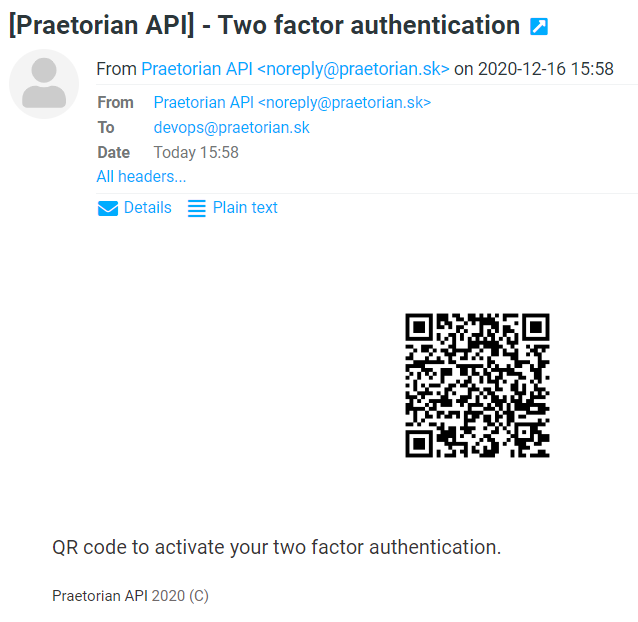
\includegraphics[width=\textwidth,height=9cm,keepaspectratio=true]{assets/2fa_email.png}\end{center}
\caption[Obsah emailu informujúcom o aktivácii dvojfaktorovej autentifikácie]{Obsah emailu informujúcom o aktivácii dvojfaktorovej autentifikácie}\label{fig:obr_14}
\end{figure}

Naskenovaním daného qr kódu, napríklad v aplikácii „Authenticator“, sa vytvorí nový účet, ktorému je priradený práve jeden OTP
s veľmi krátkou životnosťou.
Po uplynutí životnosti sa OTP automaticky pregeneruje.
Vytvorený účet v aplikácii Authenticator so zobrazeným OTP je znázornený na obrázku~\ref{fig:obr_15}.

\begin{figure}[H]
\begin{center}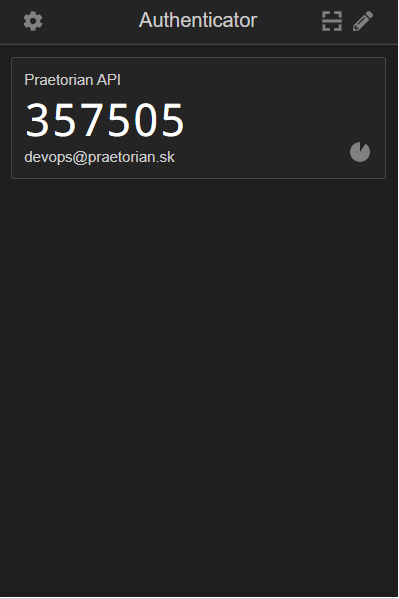
\includegraphics[width=\textwidth,height=9cm,keepaspectratio=true]{assets/authenticator.png}\end{center}
\caption[Zobrazenie aktivovaného účtu s OTP v aplikácii Authenticator]{Zobrazenie aktivovaného účtu s OTP v aplikácii Authenticator}\label{fig:obr_15}
\end{figure}

Ďalšou z možností nami vytvoreného používateľa je pripojenie sa na vzdialené zariadenie pomocou ssh proxy servera, pričom na
pripojenie je použité interaktívne prostredie.
Celý proces pripojenia používateľa ku koncovému zariadeniu je zobrazený na obrázku~\ref{fig:obr_16}

\begin{figure}[H]
\begin{center}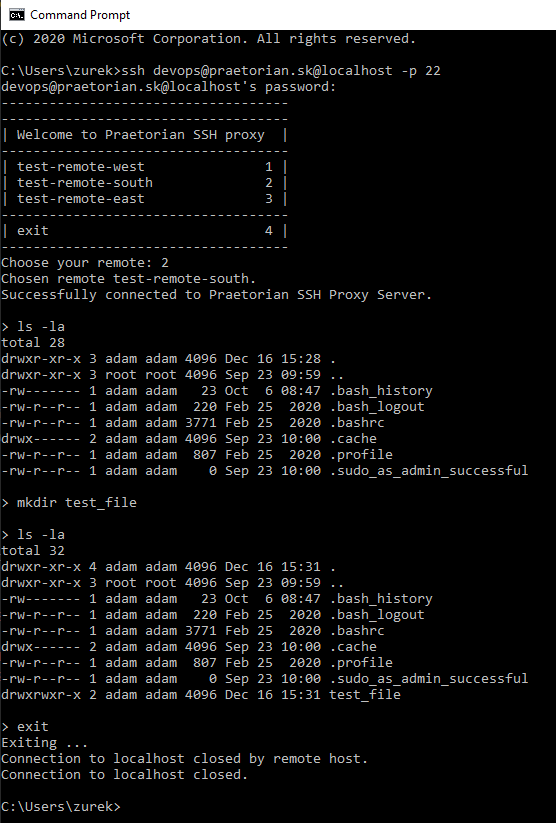
\includegraphics[width=\textwidth,height=15cm,keepaspectratio=true]{assets/interactive_session.png}\end{center}
\caption[Proces pripojenia cez interaktívne prostredie]{Proces pripojenia cez interaktívne prostredie}\label{fig:obr_16}
\end{figure}

Používateľ cez interaktívne prostredie vytvoril na koncovom zariadení priečinok s názvom „test\_file“.
Ak chce cez neinteraktívne prostredie daný priečinok zmazať, musí si v prvom rade vytvoriť skript, ktorý bude obsahovať
tri príkazy:
\newpage

\begin{enumerate}
  \item \inlinecode{ls -la}
  \item \inlinecode{rmdir log\_entries}
  \item \inlinecode{ls -la}
\end{enumerate}

Nasledovne si musí vytvoriť dočasného používateľa, ktorého úlohou bude daný skript jednorázovo vykonať, pričom bude po
dokončení úlohy dočasný požívateľ vymazaný.
Pre vytvorenie dočasného používateľa je potrebné sa prihlásiť za permanentného používateľa do webového api rozhrania a
vytvoriť nasledovnú požiadavku:

\textbf{\large Požiadavka [POST]:}

\begin{lstlisting}[language=json,firstnumber=1]
{
  "project_id": "408c57f3-6ea4-42dc-beb3-a0051b97182f",
  "remote_id": "f2228baf-d999-4d7a-9780-b8f2be97956f"
}
\end{lstlisting}

\textbf{\large Odpoveď:}

\begin{lstlisting}[language=json,firstnumber=1]
{
  "response": {
    "username": "jPTgEYC@praetorian.sk",
    "password": "AnVV6kLPA9"
  }
}
\end{lstlisting}

Používateľovi taktiež v prípade zabudnutia prístupových údajov k dočasnému používateľovi dôjde notifikácia s potrebnými
informáciami, ktorej obsah je zobrazený na obrázku~\ref{fig:obr_17}.

\begin{figure}[H]
\begin{center}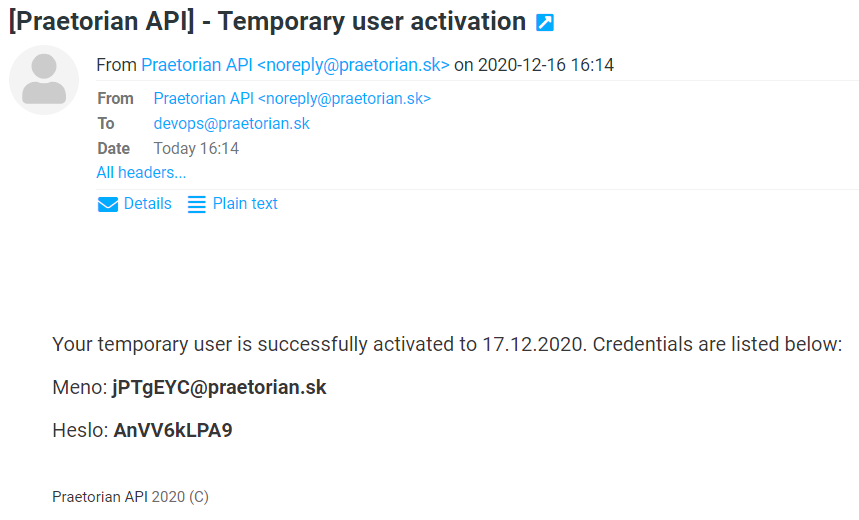
\includegraphics[width=\textwidth,height=9cm,keepaspectratio=true]{assets/temporary_credentials.png}\end{center}
\caption[Obsah emailu informujúcom o prístupových údajoch dočasného používateľa]{Obsah emailu informujúcom o prístupových údajoch dočasného používateľa}\label{fig:obr_17}
\end{figure}

Po úspešnom vytvorení skriptu a dočasného používateľa je možné sa pripojiť na koncové zariadenie cez neinteraktívne prostredie,
ktorého vykonanie je na obrázku~\ref{fig:obr_18}.

\begin{figure}[H]
\begin{center}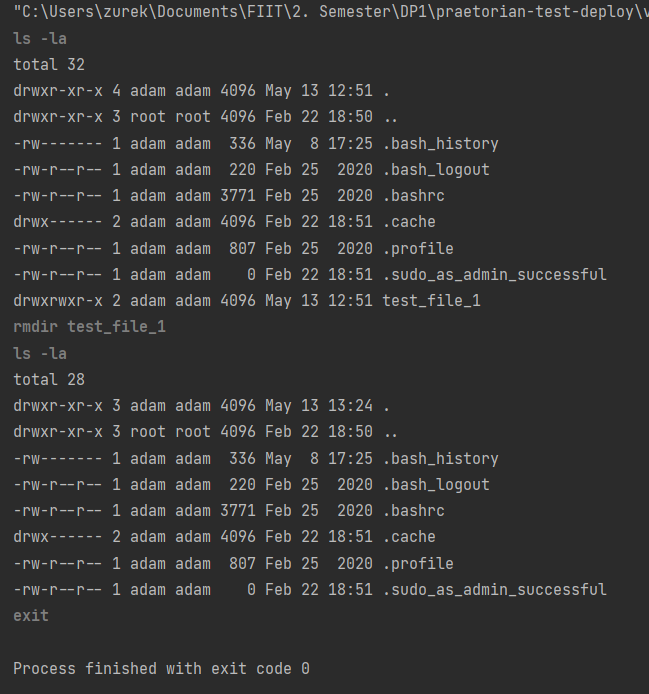
\includegraphics[width=\textwidth,height=12cm,keepaspectratio=true]{assets/non_interactive_session.png}\end{center}
\caption[Proces pripojenia cez neinteraktívne prostredie]{Proces pripojenia cez neinteraktívne prostredie}\label{fig:obr_18}
\end{figure}

Po úspešnom dokončení vykonávania príkazov na dané koncové zariadenie, bolo nasledovne ukončené spojenie a dočasný používateľ
bol vymazaný.

Dané riešenie pokrýva viacero scenárov použitia, ako napríklad manažment používateľov, projektov a skupín, monitorovanie
všetkých systémových akcií, kontrola povolených zariadení a mnoho ďalších.
No hlavnou úlohou v danej fáze riešenia bolo predovšetkým preukázať zmysel riešeného zadania preukázanou modularitou a procesom
bezpečného pripojenia na vzdialené zariadenia, ktorý je možné rozširovať o nové bezpečnostné prvky a prípady použitia.

\chapter{Zhodnotenie}\label{ch:zhodnotenie}

Prvotnou myšlienkou nášho riešenia bola predovšetkým schopnosť ukladať citlivé firemné údaje na centralizované dátové úložisko
s cieľom využitia potenciálu na automatizovanie procesov, ktoré sú voči zneužitiu z pohľadu informačnej bezpečnosti
najcitlivejšie.
Prístup k citlivým údajom podlieha určitým oprávneniam, ktoré je možné nakonfigurovať pre každú z firiem rozdielne, aby
odzrkadľovali vnútro-firemnú štruktúru.
Z dôvodu vyžadovania takejto formy prístupu u všetkých typoch firemných procesov, sme sa rozhodli využiť danú myšlienku
centralizovaného úložiska rozšírením vo forme nadstavby api rozhrania, cez ktoré bude umožnená bezpečná komunikácia s centralizovaným
úložiskom.
Týmto riešením je umožnené konfigurovať nielen vnútro-firemnú štruktúru, no taktiež manažovanie citlivých údajov a ich monitorovanie.
Keďže výsledné webové api rozhranie reprezentovalo samostatný modul, bolo možné vytvoriť ďalšie moduly s rôznymi funkcionalitami,
ako napríklad zabezpečenie prístupu na vzdialené zariadenia.
Takýto modul vie s webovým api rozhraním komunikovať a poskytuje ďalšie možné formy nadstavby, ako napríklad poskytnutie
komunikácie s vzdialenými zariadeniami.

Jedným z problémov, ktorý sa počas implementácie ssh proxy servera vyskytol, nastával pri odchytávaní príkazov v interaktívnom
móde pripojenia vzhľadom na whitelist, alebo blacklist proces filtrovania.
Jadro problému spočívalo v spôsobe implementácie, ktorá fungovala iba spôsobom presmerovania vstupov a výstupov komunikujúcich
uzlov.
Tým pádom boli z klienta na vzdialené zariadenie preposielané všetky znaky bez možnosti buffrovania vstupu, následného
rozoznania jednotlivých príkazov a následnej kontroly pred ich odoslaním na vzdialené zariadenie.
Druhý problém spočíval v kvantitatívnom vyhodnotení nášho riešenia.
Hlavnými kritériami systému je bezpečnosť, modularita, udržiavateľnosť a rozšíriteľnosť s cieľom jeho použitia softvérovou
firmou v praxi.

Existuje vysoký počet možností, ktorými je dané riešenie možné zlepšovať.
Hlavnou prioritou pri práci v ďalšej fáze projektu bude vyriešenie filtrovania v interaktívnom prostredí ssh, kde jednou
z možných riešení je rozdelenie daného prostredia na dva ďalšie typy, pričom prvý by bol promiskuitný, ktorého úlohou
by bol neobmedzený prístup bez kontroly vstupov.
Druhý by vstup ukladal do vyrovnávacej pamäte dovtedy, dokiaľ nebude poslaný znak nového riadku, alebo dokiaľ neuplynie
časový interval.
Následne by bol pred odoslaním daný vstup skontrolovaný a napokon poslaný na koncové zariadenie.
Ďalšími možnosťami zlepšenia by bolo systémové zaznamenávanie udalostí na ssh proxy serveri do syslogu, alebo dané riešenie
kvantitatívne a kvalitatívne ohodnotiť podľa penetračných testov, alebo softvérových metrík.

\chapter{Záver}\label{ch:zaver}

Prvotnou myšlienkou nášho riešenia bola predovšetkým schopnosť ukladať citlivé firemné údaje na centralizované dátové úložisko
s cieľom využitia potenciálu na automatizovanie procesov, ktoré sú voči zneužitiu z pohľadu informačnej bezpečnosti
najcitlivejšie.
Prístup k citlivým údajom podlieha určitým oprávneniam, ktoré je možné nakonfigurovať pre každú z firiem rozdielne, aby
odzrkadľovali vnútro-firemnú štruktúru.
Z dôvodu vyžadovania takejto formy prístupu u všetkých typoch firemných procesov, sme sa rozhodli využiť danú myšlienku
centralizovaného úložiska rozšírenú o nadstavbu api rozhrania.
Touto formou bude umožnená bezpečná komunikácia s centralizovaným úložiskom.
Daným riešením je tým pádom umožnené konfigurovať nielen vnútro-firemnú štruktúru, no taktiež manažovanie citlivých údajov a ich monitorovanie.
Keďže výsledné webové api rozhranie reprezentovalo samostatný modul, bolo možné vytvoriť ďalšie moduly s rôznymi funkcionalitami.
Modul vo forme ssh proxy servera vie s webovým api rozhraním komunikovať a poskytuje ďalšie možné formy nadstavby,
ako napríklad poskytnutie komunikácie so vzdialenými zariadeniami.
Ďalším rozšírením bolo zabezpečenie komunikácie implementáciou api klienta, ktorý bol všestranne využívaný naprieč rozličnými
modulmi riešenia.
Posledným rozšírením bola nadstavba knižnice fabric, pre nami špecifikovanú komunikáciu, ktorá slúžila ako ukážka rozšírenia
ktoréhokoľvek nástroja tohto typu bez ohľadu na použitý programovací jazyk, alebo technológiu.
Kľúčovým bodom výskumu bolo navrhnutie a implementácia komunikácie medzi dvoma uzlami, ktoré sú medzi sebou anonymizované za
pomoci tretej strany.
Medzi zariadeniami by bolo možné posielať rôzne citlivé, prístupové a konfiguračné údaje bez nutnosti používateľa k nim
akýmkoľvek spôsobom pristúpiť.
Všetky tieto operácie museli podliehať striktnou kontrolou bezpečnosti, aby bolo dané riešenie možné využívať v praxi softvérovými firmami.
Systém bol navrhovaný a implementovaný dodržiavaním kritérií, ako bezpečnosť, modularita, udržiavateľnosť, rozšíriteľnosť
a auditovateľnosť.

Jedným z problémov, ktorý sa počas implementácie ssh proxy servera vyskytol, nastával pri odchytávaní príkazov v interaktívnom
móde pripojenia vzhľadom na whitelist, alebo blacklist proces filtrovania.
Jadro problému spočívalo v spôsobe implementácie, ktorá fungovala iba spôsobom presmerovania vstupov a výstupov komunikujúcich
uzlov.
Tým pádom boli z klienta na vzdialené zariadenie preposielané všetky znaky bez možnosti buffrovania vstupu, následného
rozoznania jednotlivých príkazov a následnej kontroly pred ich odoslaním na vzdialené zariadenie.

\section{Vízia}\label{sec:vizia}

Existuje značný počet možností, ktorými je dané riešenie možné rozširovať a upravovať jeho stávajúce funkcionality.
Medzi najvyššie priority patrí používateľské grafické rozhranie pre správu jednotlivých častí systému.
Rozdeľovalo by sa na dve časti, kde prvou by bolo administrátorské rozhranie spravujúce tie najviac dôverné súčasti systému,
ako napríklad: Prístupové údaje, pridávanie projektov, asociácia koncových zariadení do projektov správa práv používateľov a iné.
Druhou časťou by bolo rozhranie zamestnancov, ktorým by bolo umožnené prehliadať asociované projekty, koncové zariadenia, možnosti
prístupov a mieru operácií, ktoré môžu na danom projekte, alebo zariadení vykonať.
Grafické rozhranie by mohlo byť implementované v podobe webovej stránky, alebo mobilnej aplikácie.
Čo sa týka úpravy stávajúcej funkcionality, anonymizovaná komunikácia by mohla byť využitá na dynamickú zmenu prístupových údajov
na koncové zariadenia v určitých časových intervaloch, čím by sa minimalizovalo riziko odchytenia a dešifrovania aktuálnych
prístupových údajov pomocou MITM útoku.
Pre ssh proxy server by bolo potrebné rozšíriť formu autentifikácie pomocou RSA kľúčov a upraviť kontrolu zariadení používateľov
pomocou SSL certifikátov.
Autorizácia by sa mohla rozšíriť o kontrolu prístupu používateľov k jednotlivým koncovým zariadeniam pre jednotlivé projekty,
čo bolo spomínané aj v štvrtej kapitole: Návrh riešenia.
Pre zvýšenie miery kontroly a bezpečnosti je možné pridanie overenia druhu siete, z ktorej sa používateľ pripája a tým zabrániť
pripojenie z verejných sietí mimo lokálnej siete firmy, alebo vpn.
Autentifikáciu je možné rozšíriť pre podporu LDAP rozhrania.
Počas komunikácie medzi zariadením používateľa a koncovým zariadením zákazníka by ssh proxy server mohol filtrovať nežiadúce príkazy
pomocou metódy whitelist, alebo blacklist.


% Bibliography
\printbibliography[heading=references,segment=\therefsegment]
\addcontentsline{toc}{chapter}{Zoznam použitej literatúry}

% no page numbers for appendicies
\addtocontents{toc}{\protect\setcounter{tocdepth}{0}}
\addtocontents{toc}{\cftpagenumbersoff{chapter}}

\end{refsegment}

\appendix
\chapter{Plán práce}

\pagenumbering{arabic}
\renewcommand*{\thepage}{A\arabic{page}}

\section{Zimný semester}

\begin{tabular}{|l||l|}
\hline
1. - 4. týždeň & Konzultácie a hľadanie súvisiaceho výskumu  \\
\hline
5. - 6. týždeň & Práca na úvode a analýze práce  \\
\hline
7. týždeň & Konzultácie  \\
\hline
8. - 10. týždeň & Práca na sekcii existujúce riešenia  \\
\hline
11. týždeň & Úpravy a práca na zhodnotení analýzy \\
\hline
12. týždeň & Finálne konzultácie pred odovzdaním \\
\hline
\end{tabular}

\section{Letný semester}

\begin{tabular}{|l||l|}
\hline
1. - 2. týždeň & Úprava v analýze práce \\
\hline
3. - 6. týždeň & Navrhovanie riešenia a implementácia webového api rozhrania\\
\hline
7. - 9. týždeň & Navrhovanie riešenia a implementácia ssh proxy servera \\
\hline
10. týždeň & Konzultácie a opravy v implementácii  \\
\hline
11. - 12. týždeň & Spísanie finálneho dokumentu a následné konzultácie  \\
\hline
\end{tabular}

\renewcommand\chaptername{Príloha}

\chapter{Obsah priloženého elektronického média}

\renewcommand*{\thepage}{B\arabic{page}}
\setcounter{page}{1}

V priloženej prílohe sa nachádza:

\begin{itemize}
    \item Diplomový projekt vo formáte PDF (v koreňovom adresári).
    \item Implementácia webového api rozhrania (v adresári api).
    \item Implementácia ssh proxy servera (v adresári proxy).
    \item Implementácia api klienta (v adresári klient).
    \item Implementácia nadstavby knižnice fabric (v adresári fabric).
    \item Implementácia testovacieho projektu na nasadzovanie (v adresári deploy).
    \item Dokumentácia k REST API vo formáte PDF (v adresári docs).
    \item Odkazy na github repozitáre projektov (v súbore odkazy.txt)
\end{itemize}

\renewcommand\chaptername{Príloha}

\chapter{Používateľská príručka}

\renewcommand*{\thepage}{C\arabic{page}}
\setcounter{page}{1}

Príručka obsahuje informácie o postupe inštalácie systému, jeho konfigurácie a používania.

Celý systém je rozdelený na päť častí, ktoré sa nachádzajú v priloženom elektronickom médiu.
Riešenia \inlinecode{praetorian-api-client} a \inlinecode{praetorian-fabric} slúžia, ako knižnice používané v iných súčastiach systému.
Tým pádom ich nie je potrebné inštalovať, konfigurovať ani spúšťať.
Napriek tomu sa dodatočné informácie o daných knižniciach nachádzajú v súbore \emph{README.md} sídliacom v koreňovom adresári projektu.

Čo sa týka projektu \inlinecode{praetorian-test-deploy}, ten slúži na testovacie účely, ako forma vyvýjaného produktu
obsahujúceho potrebné skripty na komunikáciu s koncovými zariadeniami.

Z týchto dôvodov je príručka podľa dvoch hlavných komponentov systému, čo sú \inlinecode{praetorian-api} a \inlinecode{praetorian-ssh-proxy} rozdelená na iba dve časti.


\section{Praetorian API}

Projekt slúži, ako api server komunikujúci so zariadením používateľa prostredníctvom HTTPS REST komunikácie.
Riešenie obsahuje správu a manažment všetkých entít v systéme.

\subsection{Inštaláca}

Na spustenie daného riešenia je potrebné si nainštalovať:

\begin{enumerate}
\item Programovací jazyk \inlinecode{python 3.7+}:
\begin{itemize}
\item \emph{https://www.python.org/downloads/}
\end{itemize}
\item Relačnú databázu \inlinecode{PostgreSql 12}:
\begin{itemize}
\item \emph{https://www.postgresql.org/download/}
\end{itemize}
\end{enumerate}

Ďalším krokom je vytvorenie virtuálneho prostredia a inštalácia package manažéra \inlinecode{poetry} pre konkrétny projekt pomocou príkazov:
\begin{itemize}
\item \inlinecode{python -m venv venv}
\item \inlinecode{pip install poetry}
\end{itemize}

Posledným krokom inštalácie je inštalácia závislostí pomocou príkazu:
\begin{itemize}
\item \inlinecode{poetry install}
\end{itemize}

\subsection{Konfigurácia}

Pre nastavenie pripojenia databázy PostgreSQL je potrebné vytvoriť súbor \inlinecode{.env}, kde budú nastavené environment
premenné podľa ukážky v súbore \inlinecode{.env.example}.
\newpage

Inicializácia databázy je vykonaná nasledujúcimi príkazmi:
\begin{itemize}
\item \inlinecode{python manage.py migrate}
\item \inlinecode{python manage.py sync\_roles}
\end{itemize}

Na vytvorenie prvého používateľa v systéme s administrátorskými právami je potrebné vykonať nasledujúci príkaz:
\begin{itemize}
\item \inlinecode{python manage.py createsuperuser}
\end{itemize}

\subsection{Návod}

Projekt je možné spustiť príkazom:
\begin{itemize}
\item \inlinecode{python manage.py runserver [HOST]:[PORT]}
\item Príklad: \inlinecode{python manage.py runserver localhost:8000}
\end{itemize}

Pre volanie požiadaviek na spustený api server je potrebné si nainštalovať jednu z platform pre vývoj API, ako napríklad:

\begin{enumerate}
\item \inlinecode{Postman}:
\begin{itemize}
\item \emph{https://www.postman.com/downloads/}
\end{itemize}
\end{enumerate}

Celá REST API dokumentácia vo formáte PDF s príkladmi požiadaviek a odpovedí sa nachádza v obsahu priloženého média v
adresári \emph{docs}.

\section{Praetorian SSH Proxy}

Daný projekt slúži, ako tretia strana zastrešujúca komunikáciu medzi zariadením používateľa a koncovým zariadením zákazníka.
Komunikácia prebieha aj medzi proxy serverom a api serverom pomocou api klienta.

\subsection{Inštaláca}

Na spustenie daného riešenia je potrebné si nainštalovať:

\begin{enumerate}
\item Programovací jazyk \inlinecode{python 3.8+}:
\begin{itemize}
\item \emph{https://www.python.org/downloads/}
\end{itemize}
\end{enumerate}

Ďalším krokom je vytvorenie virtuálneho prostredia a inštalácia package manažéra \inlinecode{poetry} pre konkrétny projekt pomocou príkazov:
\begin{itemize}
\item \inlinecode{python -m venv venv}
\item \inlinecode{pip install poetry}
\end{itemize}

Posledným krokom inštalácie je inštalácia závislostí pomocou príkazu:
\begin{itemize}
\item \inlinecode{poetry install}
\end{itemize}

\subsection{Konfigurácia}

Pre nastavenie pripojenia na api server je potrebné vytvoriť súbor \inlinecode{.env}, kde budú nastavené environment
premenné podľa ukážky v súbore \inlinecode{.env.example}.

\subsection{Návod}

Projekt je možné spustiť príkazom:
\begin{itemize}
\item \inlinecode{python run.py [HOST] [PORT]}
\item Príklad: \inlinecode{python run.py localhost 22}
\end{itemize}

\newpage

Na koncové zariadenie pomocou interaktívneho session je možné sa pripojiť príkazom:
\begin{enumerate}
    \item Nepriamy spôsob:
    \begin{itemize}
        \item \inlinecode{ssh [USERNAME]@[HOST] -p [PORT]}
        \item Príklad: \inlinecode{ssh user@praetorian.sk@localhost -p 22}
    \end{itemize}
    \item Priamy spôsob:
    \begin{itemize}
        \item Priame: \inlinecode{ssh [USERNAME]+[PROJECT]-[REMOTE]@localhost -p 22}
        \item Príklad: \inlinecode{ssh user@praetorian.sk+Project-Remote@localhost -p 22}
    \end{itemize}
\end{enumerate}

Na pripojenie sa ku koncovému zariadeniu pomocou neinteraktívneho session je potrebný projekt s nainštalovanou rozšírenou
knižnicou fabric.
Pre otestovanie tohto spôsobu je možné otvoriť spomínaný \inlinecode{praetorian-test-deploy} projekt v ktorého README.md súbore
sa nachádzajú všetky potrebné informácie.
Po vytvorení skriptu je možné zavolať neinteraktívny session príkazom:

\begin{itemize}
\item \inlinecode{fab [FUNCTION] [REMOTE]}
\item Príklad: \inlinecode{fab deploy production}
\end{itemize}


\end{document}
